\documentclass[12pt]{article}
\usepackage[utf8]{inputenc}
\usepackage{longtable}
\usepackage{color}
\usepackage{multirow}
\usepackage{hyperref}
\usepackage{amssymb}
\usepackage{setspace}
%\doublespacing

\renewcommand*{\sectionautorefname}{Section} 

\title{Predation model \\ Hybridisation\_A} 
\author{Raphael Klein, EPFL}

\usepackage{natbib}
\usepackage{graphicx}
\usepackage[labelfont=bf]{caption} 	% Make captions bold (Figure & Table)
\usepackage{subfig}	
\usepackage{amsmath}
\usepackage{hyperref}
%\usepackage[section]{placeins}

\providecommand{\keywords}[1]{\textbf{Keywords:} #1}

\begin{document}

\maketitle

%\textcolor{red.green.blue.cyan.yellow.magenta.}{}

This reports the hybridisation of the predation model with the ACF implementation of the policy model. It outlines how the models were hybridised and goes through the initialisation of the models and the experiments that will be run using these models.

\tableofcontents

%%%%%%%%%%%%%%%%%%%%%%%%%%%%%%%%%%%%%%%%%%%%%%%%%%%%%%%%%%%%%%%%%%
\section{The problem tree}
\label{sec:interfaceProblemTree}
%%%%%%%%% %%%%%%%%%%%%%%%%%%%%%%%%%%

Overall, the problem tree is given as follows:

\begin{itemize}
\item Policy core problems:
	\begin{enumerate}
	
	\item Sheep - 
	The amount of sheep on the grid.
	
	\item Wolf - 
	The amount of wolves on the grid.
	
	\item Fully grown grass - 
	The amount of fully grown grass on the grid.
	
	\end{enumerate}
	
\item Secondary problems:
	\begin{enumerate}

	\item Net sheep population change - 
	This is the difference between initial and final amount of sheep.
	
	\item Net wolf population change - 
	This is the difference between initial and final amount of wolves.
	
	\item Net grown grass patch change - 
	This is the difference between initial and final amount of grown grass patches.
	
	\end{enumerate}
	
\end{itemize}

Note that the secondary issues and the policy core issues are the same. The main reason behind this choice is the simplicity of the model. The model is so simple that the it is difficult to find any different policy core issues.

%%%%%%%%%%%%%%%%%%%%%%%%%%%%%%%%%%%%%%%%%%%%%%%%%%%%%%%%%%%%%%%%%%
\section{The policy instruments}
\label{sec:interfaceInstruments}
%%%%%%%%% %%%%%%%%%%%%%%%%%%%%%%%%%%

The policy instruments within the policy tree are implemented using incremental increases and decreases in the following exogenous parameters.

\begin{enumerate}
\item Change sheep reproduction [CR-0.01/+0.01]
\item Change wolf reproduction [WR -0.01/+0.01]
\item Change grass regrowth [GR-2/+2]
\end{enumerate}



%%%%%%%%%%%%%%%%%%%%%%%%%%%%%%%%%%%%%%%%%%%%%%%%%%%%%%%%%%%%%%%%%%
\section{The steps for model integration}
\label{sec:steps}
%%%%%%%%% %%%%%%%%%%%%%%%%%%%%%%%%%%

This section presents the steps that are needed to connect a policy context model, in this case the predation model, to the policy process model.

\begin{enumerate}
\item Before any coding, define what the belief tree and the policy instruments will be for the predation model.
\item Copy the policy emergence model files into the same folder.
\item In \texttt{runbatch.py}, replace the policy context items by the predation model.
\item In \texttt{runbatch.py}, make sure to initialise the predation model appropriately.
\item Change the \texttt{input goalProfiles} files to have the appropriate belief tree structure of the predation model.
\item In \texttt{model module interface.py}, construct the belief tree and the policy instrument array.
\item Make sure that the step function in the \texttt{model predation.py} returns the KPIs that will fit in the belief system in the order DC, PC and S. If no DC is considered, then include one value of 0 at least. All KPIs need to be normalised.
\item Modify the step function of the \texttt{model predation.py} to include a policy implemented.
\item Introduce the changes that a policy implemented would have on the model in \texttt{model predation.py}.
\end{enumerate}


%%%%%%%%%%%%
\subsection{Code documentation}

The following is the documentation for the hybrid model. This includes the script files that are needed to connect the policy context model (electricity model in the present case) with the policy emergence model.


\paragraph{run\_batch.py}

This script is used to simulate the entire hybrid model for different scenario. To this effect, it contains the inputs for all models. This includes the inputs for the hybrid model itself (number of steps, duration of steps, number of repetitions, number of scenarios, ...), the inputs for the policy context, and the inputs for the policy emergence model (actor distribution, actor belief profiles, ...)

This is then followed by the for loop that simulate the hybrid model. This includes the simulation of a warm up round. Then the policy context is simulated n times for every policy process step simulation. Each feeds the other through indicators and policy selection. The results are all extracted using the data collector from each of the model. The files are saved within .csv files.

\paragraph{model\_module\_interface.py}

This script is used to connect the policy context to the policy emergence model. This part of the model will change every time a new policy context is considered. For this, two functions are considered:

\begin{itemize}
\item \texttt{belief\_tree\_input()}

This function is used to define the agent issue tree. It includes the specification of the deep core, policy core and secondary issues.

\item \texttt{policy\_instrument\_input()}

This function is used to define the policy instruments that the agents can select.

\end{itemize}



%%%%%%%%%%%%%%%%%%%%%%%%%%%%%%%%%%%%%%%%%%%%%%%%%%%%%%%%%%%%%%%%%%
\section{The steps for model simulation}
\label{sec:steps}
%%%%%%%%% %%%%%%%%%%%%%%%%%%%%%%%%%%

This section presents the steps that are needed to connect a policy context model, in this case the predation model, to the policy process model.

\begin{enumerate}
\item For the policy process:
	\begin{enumerate}
	\item Define a set of hypotheses to be tested
	\item Define scenarios that will be needed to assess the hypotheses
	\item Choose the agent distribution based on the scenarios constructed
	\item Set the preferred states for the active agents and the electorate along with the causal beliefs to be used. This should all be based on the scenarios that have been constructed.
	\end{enumerate}

\item For the predation model:
	\begin{enumerate}
	\item Define the initial values for the main parameters
	\item Define the parameters that will be recorded
	\end{enumerate}
\item Save the right data from the model.
\end{enumerate}

%%%%%%%%%%%%%%%%%%%%%%%%%%%%%%%%%%%%%%%%%%%%%%%%%%%%%%%%%%%%%%%%%%
\section{Model hypotheses}
\label{sec:hypotheses}
%%%%%%%%% %%%%%%%%%%%%%%%%%%%%%%%%%%

Because of the complexity of the model, there are a lot of hypotheses that can be tested with this ACF policy emergence model. However, we will try not to demonstrate the same hypotheses that were demonstrated for the SM. This would be redundant. This includes all of the hypotheses that establish a causal relation between policy change and environment change. The focus will instead be placed on the impact that the new elements, for each of the model variations, has on policy change and on the dynamics of the model. This includes the impact of policy learning and coalitions on policy change.

%%%%%%%%%%%%%%%%%%%%%%%%%%%%%%%%%%%%%%%%%%%%%%%%%%%%%%%%%%%%%%%%%%
\subsection{The +PL model}

The main research question that we want to answer with this model is:

\emph{What impact does policy learning have on policy change within the ACF+PL model?}

Several hypotheses are considered to answer this question:

\begin{itemize}
\item H1: Policy learning leads to policy change.
\item H2: The resources distribution will affect the speed and the direction of policy learning.
\item H4: The balance of power will affect the speed and the direction of policy learning.
\end{itemize}

%%%%%%%%%%%%%%%%%%%%%%%%%%%%%%%%%%%%%%%%%%%%%%%%%%%%%%%%%%%%%%%%%%
\subsection{The +Co model}

The main research question that we want to answer with this model is:

\emph{What impact do coalitions have on policy change within the ACF+Co model?}

Several hypotheses are considered to answer this question:

\begin{itemize}
\item H1: Broader coalitions will normalise all of the beliefs around its dominant belief.
\item H2: Powerful but restrictive coalition will influence strongly other agents until they are in the same coalition.
\end{itemize}


%%%%%%%%%%%%%%%%%%%%%%%%%%%%%%%%%%%%%%%%%%%%%%%%%%%%%%%%%%%%%%%%%%
\section{Model scenarios}
\label{sec:steps}
%%%%%%%%% %%%%%%%%%%%%%%%%%%%%%%%%%%

We differentiate the scenarios that will be run for the +PL and the +Co models within this section. For each scenario, we have to consider the belief system of the agents, the agent distribution and the resource distribution. Though in the formalisation of the model we do not make a mention of affiliations (except when it comes to the electorate influence), we will still use affiliations here to simplify the initialisation of the agents for the policy emergence model.

%%%%%%%%%%%%%%%%%%%%%%%%%%%%%%%%%%%%%%%%%%%%%%%%%%%%%%%%%%%%%%%%%%
\subsection{The +PL model}

For now only the benchmark scenario and scenario 1 are considered. These basically test the different impact of a change of resources on policy learning and the associated effect on policy change, if any. For each of the scenario, the preferred states of the agents are shown in \autoref{tab:preferredStates}, their causal relations are provided in \autoref{tab:causalBeliefs} and the agents and resources distribution are provided in \autoref{tab:agentResourceDistribution}.

Note that for now we only allow the agents to influence one another on their preferred states and not on their causal beliefs.


\begin{itemize}
\item Scenario 0 - No interactions

Scenario 0 is a scenario where no interactions are taken into account. It is the SM simulation. This is used to compare with the results from the model with the interactions introduced.


\item Scenario 1 - Benchmark interactions

The benchmark scenario is to be used as a benchmark. It is a simulation of the predation model with the policy emergence model. Two affiliations are considered. Affiliation 0 consists of two policy makers and four policy entrepreneurs (2 PM and 4 PE) with high resources and a preference for sheep favouring policies. Affiliation 1 consists of one policy maker and four policy entrepreneurs (1 PM and 4 PE) with low resources and a preference for wolf favouring policies. The preferred states for the agents are provided in \autoref{tab:preferredStates}. The causal beliefs used as given in \autoref{tab:causalBeliefs}.

\item Scenario 2 - Different resource distribution

Have a simulation where the resources distribution is 99 (affiliation 1) to 1 (affiliation 0). This makes one affiliation dominating, the minority one. Observe where the policy learning ends up and see whether that ends up affecting the policy instruments being selected.

\item Scenario 3 - External event on a preferred state (policy core)

Introduce an external event on one of the preferred states of all agents to influence their beliefs and observe whether that makes a difference in their choice of policy selection. This external events happens after tick 4.

\item Scenario 4 - External event on a preferred state (secondary issue)

Introduce an external event on one of the preferred states of all agents to influence their beliefs and observe whether that makes a difference in their choice of policy selection. This external events happens after tick 4.

\item Scenario + (for the +PL scenario) - not discussed here

Future scenarios could also explore the influence of the electorate on actors with more resources. It could look at how a change in the actor distribution might have an impact on the outcomes of the simulation.

\end{itemize}

%%%%%%%%%%%%%%%%%%%%%%%%%%%%%%%%%%%%%%%%%%%%%%%%%%%%%%%%%%%%%%%%%%
\subsection{The +Co model}

The coalitions introduce three new parameters mainly: a creation coherence parameters that defines the threshold of belief difference for the creation of new coalitions, a parameter that defines the amount of resources that agents provide to coalitions they are joining, and a parameter that defines which policy core issue is the issue that coalitions assemble around. These are all varied in the following scenarios. 

\begin{itemize}
\item Scenario 5 - Coalition benchmark

The first scenario considered for the +Co model is seen as a benchmark and will be used to check it against the model without coalitions. The policy core issue of interest is the sheep one (PC0), the threshold for coalition creation is set at 0.15 and the amount of resources shared with a coalition is set to 50\% for agents that join coalitions.

\item Scenario 6 - Coalition different PC interest

The second coalition scenario changes the policy core issue of interest to the wolf one (PC1). The rest of the parameters stay the same: the threshold for coalition creation is set at 0.15 and the amount of resources shared with a coalition is set to 50\% for agents that join coalitions.

\item Scenario 7 - Coalition different PC interest

The third coalition scenario changes the policy core issue of interest to the grass one (PC2). The rest of the parameters stay the same: the threshold for coalition creation is set at 0.15 and the amount of resources shared with a coalition is set to 50\% for agents that join coalitions.

\item Scenario 8 - Coalition LHS

For this last scenario, the two coalition parameters are jumbled with a LHS algorithm. The range for the coalition creation threshold is between 0.01 and 0.25 while the range for the resources shared is set between 5\% and 75\%. A LHS algorithm is used to create 50 different inputs normally distributed. This simulation will then be repeated only 10 times to generate a total of 500 runs.

\end{itemize}

%%%%%%%%%%%%%%%%%%%%%%%%%%%%%%%%%%%%%%%%%%%%%%%%%%%%%%%%%%%%%%%%%%
\subsection{The +PK model}

The partial knowledge model is only partially tested both with the benchmark policy learning scenario and the benchmark coalition scenario.

\begin{itemize}
\item Scenario 9 - PK with +PL
\item Scenario 10 - PK with +Co
\end{itemize}

%%%%%%%%%%%%%%%%%%%%%%%%%%%%%%%%%%%%%%%%%%%%%%%%%%%%%%%%%%%%%%%%%%
\subsection{The +PI model}

% max sheep: [0, 500]
% max wolves: [0, 500]
% mass grass patches: [2500]
% Net sheep population change: [-100; 100]
% Net wolf population change: [-100; 100]
% Net grown grass patch change: [-500; 500]

\begin{table}[h!]
\begin{center}
\begin{tabular}{ |c|c|c|c|c|c|c| } 
\hline

			& {\bfseries PC1}
					&  {\bfseries PC2}
							&  {\bfseries PC3}
									&  {\bfseries S1}	
											&  {\bfseries S2}	
													&  {\bfseries S3}  	\\ 
			& Sheep	& Wolves	& Grass	& Sheep	& Wolves	& Grass 	\\
			&		&		&		& growth	& growth	& growth	\\ \hline \hline \hline
\multicolumn{7}{|c|}{ {\bfseries Scenario 0/1/2/5/6/7/8/9/10}}				\\ \hline \hline	
\multicolumn{7}{|c|}{Affiliation 0 - Pro sheep}							\\ \hline 
Value		& 400	& 50		& 2000	& 75		& -50	& 200	\\ \hline
Norm.		& 0.80	& 0.10	& 0.80	& 0.88	& 0.25	& 0.70	\\ \hline
\multicolumn{7}{|c|}{Affiliation 1 - Pro wolves}							\\ \hline 
Value		& 200	& 175	& 1700	& 50		& 25		& 120	\\ \hline
Norm.		& 0.40	& 0.35	& 0.68	& 0.75	& 0.63	& 0.62	\\ \hline
\multicolumn{7}{|c|}{ {\bfseries Scenario 3 (after)}}						\\ \hline \hline	
\multicolumn{7}{|c|}{Affiliation 0 - Pro sheep}							\\ \hline 
Value		& 50	 	& 50		& 250	& 75		& -50	& 200	\\ \hline
Norm.		& 0.10	& 0.10	& 0.10	& 0.88	& 0.25	& 0.70	\\ \hline
\multicolumn{7}{|c|}{ {\bfseries Scenario 4 (after)}}						\\ \hline \hline	
\multicolumn{7}{|c|}{Affiliation 0 - Pro sheep}							\\ \hline 
Value		& 400	& 50		& 2000	& -80	& -50	& 200	\\ \hline
Norm.		& 0.80	& 0.10	& 0.80	& 0.10	& 0.25	& 0.70	\\ \hline

\end{tabular}
\end{center}
\caption{Preferred states for the policy makers on a the interval [0,1] for scenarios 0 and 1.}
\label{tab:preferredStates}
\end{table}

\begin{table}[h!]
\begin{center}
\begin{tabular}{ |c|c|c|c|}
\hline
\multicolumn{4}{|c|}{ {\bfseries Scenario 0/1/2/3/4/5/6/7/8/9/10}}	
								\\ \hline \hline
	& PC1	& PC2	& PC3		\\ \hline
-S1 	& 1.00	& 0.75	&-0.75		\\ \hline
-S2 	&-0.75	& 1.00	& 0.25 		\\ \hline
-S3 	& 0.50	& 0.75	& 1.00		\\ 
\hline
\end{tabular}
\end{center}
\caption{Causal beliefs for the policy makers. These causal relations can be read as: an increase of 1 in S2 will lead to a decrease of 0.75 in PC1. They are all given on the interval [-1,1].}
\label{tab:causalBeliefs}
\end{table}

\begin{table}[h!]
\begin{center}
\begin{tabular}{ |l||c|c||c|c||c|c||c|c||c|c| } 
\hline
 {\bfseries Scenarios}
 				& \multicolumn{2}{|c||}{ {\bfseries 0/1/3/4/5/6/7/8}}	
						& \multicolumn{2}{|c||}{ {\bfseries 2}}	
														\\ \hline \hline
Affiliations			& 0	& 1	& 0	& 1		\\ \hline
Policy makers 		& 2	& 1	& 2	& 1		\\ \hline
Policy entrepr.		& 4	& 4	& 4	& 4		\\ \hline
Resources		& 75	& 25	& 10	& 100	\\ \hline
\end{tabular}
\end{center}
\caption{Agents and resource distribution for each of the scenarios.}
\label{tab:agentResourceDistribution}
\end{table}


\begin{table}[h!]
\begin{center}
\begin{tabular}{ |c|c|c|c|c|c|c| } 
\hline

			& {\bfseries PC1}
					&  {\bfseries PC2}
							&  {\bfseries PC3}
									&  {\bfseries S1}	
											&  {\bfseries S2}	
													&  {\bfseries S3}  	\\ 
			& Sheep	& Wolves	& Grass	& Sheep	& Wolves	& Grass 	\\
			&		&		&		& growth	& growth	& growth	\\ \hline \hline \hline
\multicolumn{7}{|c|}{ {\bfseries Scenario 11}}				\\ \hline \hline	
Affiliation 0	& 5		& 0		& 5		& 5		& 0		& 5		\\ \hline
Affiliation 1	& 5		& 5		& 5		& 5		& 5		& 5		\\ \hline

\end{tabular}
\end{center}
\caption{Biased values for the external parties for the +PI add-on scenarios. For a value of 5, the external party informs itself directly from the truth agent. For a value of 0, the external party does not change its beliefs.}
\label{tab:biasPI}
\end{table}


%%%%%%%%%%%%%%%%%%%%%%%%%%%%%%%%%%%%%%%%%%%%%%%%%%%%%%%%%%%%%%%%%%
\section{Initialisation of the model}
\label{sec:initialisation}
%%%%%%%%%%%%%%%%%%%%%%%%%%%%%%%%%%%

%%%%%%%%%%%%
\subsection{The predation model}

The parameters that need to be initialised for the predation model are given by:

\begin{itemize}
\item Grid height: 50
\item Grid width: 50
\item Initial amount of grass: about 50\% of the grid
\item Initial number of sheep: 250
\item Sheep reproduce rate: 4\%
\item Sheep gain from food: 6
\item Initial number of wolves: 25
\item Wolf reproduce rate: 5\%
\item Wolf gain from food: 35
\item Grass regrowth time: 30
\end{itemize}

Note that the initial parameter as chosen such that if only the predation model is run, it has a stable configuration. Furthermore the onus is placed on the simulation of the policy process, therefore no scenarios are placed on the predation model side of the simulation.


%%%%%%%%%%%%
\subsection{The policy process model}

%%%%%%%%%%%%
\subsection{The hybrid model}

Conflict level thresholds ...

Resources spent


%%%%%%%%%%%%%%%%%%%%%%%%%%%%%%%%%%%%%%%%%%%%%%%%%%%%%%%%%%%%%%%%%%
\section{Results}
\label{sec:}
%%%%%%%%%%%%%%%%%%%%%%%%%%%%%%%%%%%

There are a number of results we can look at:

\begin{enumerate}
\item Predation model results (count of sheep and wolves)
\item Policy selection
\item Belief evolution (both policy core and secondary preferred states) per affiliation of course - This is the new part in this part of the simulation - This can be used to track the policy learning happening within the system.
\end{enumerate}

The figures are presented in an order that builds the model with first the preferred state evolution and then selection of the policy core issues. This is followed by the preferred state evolution and then selection of the secondary issues. This is followed by the policy instrument selection, and then the outcome changes in the predation model.

\begin{figure}
\centering
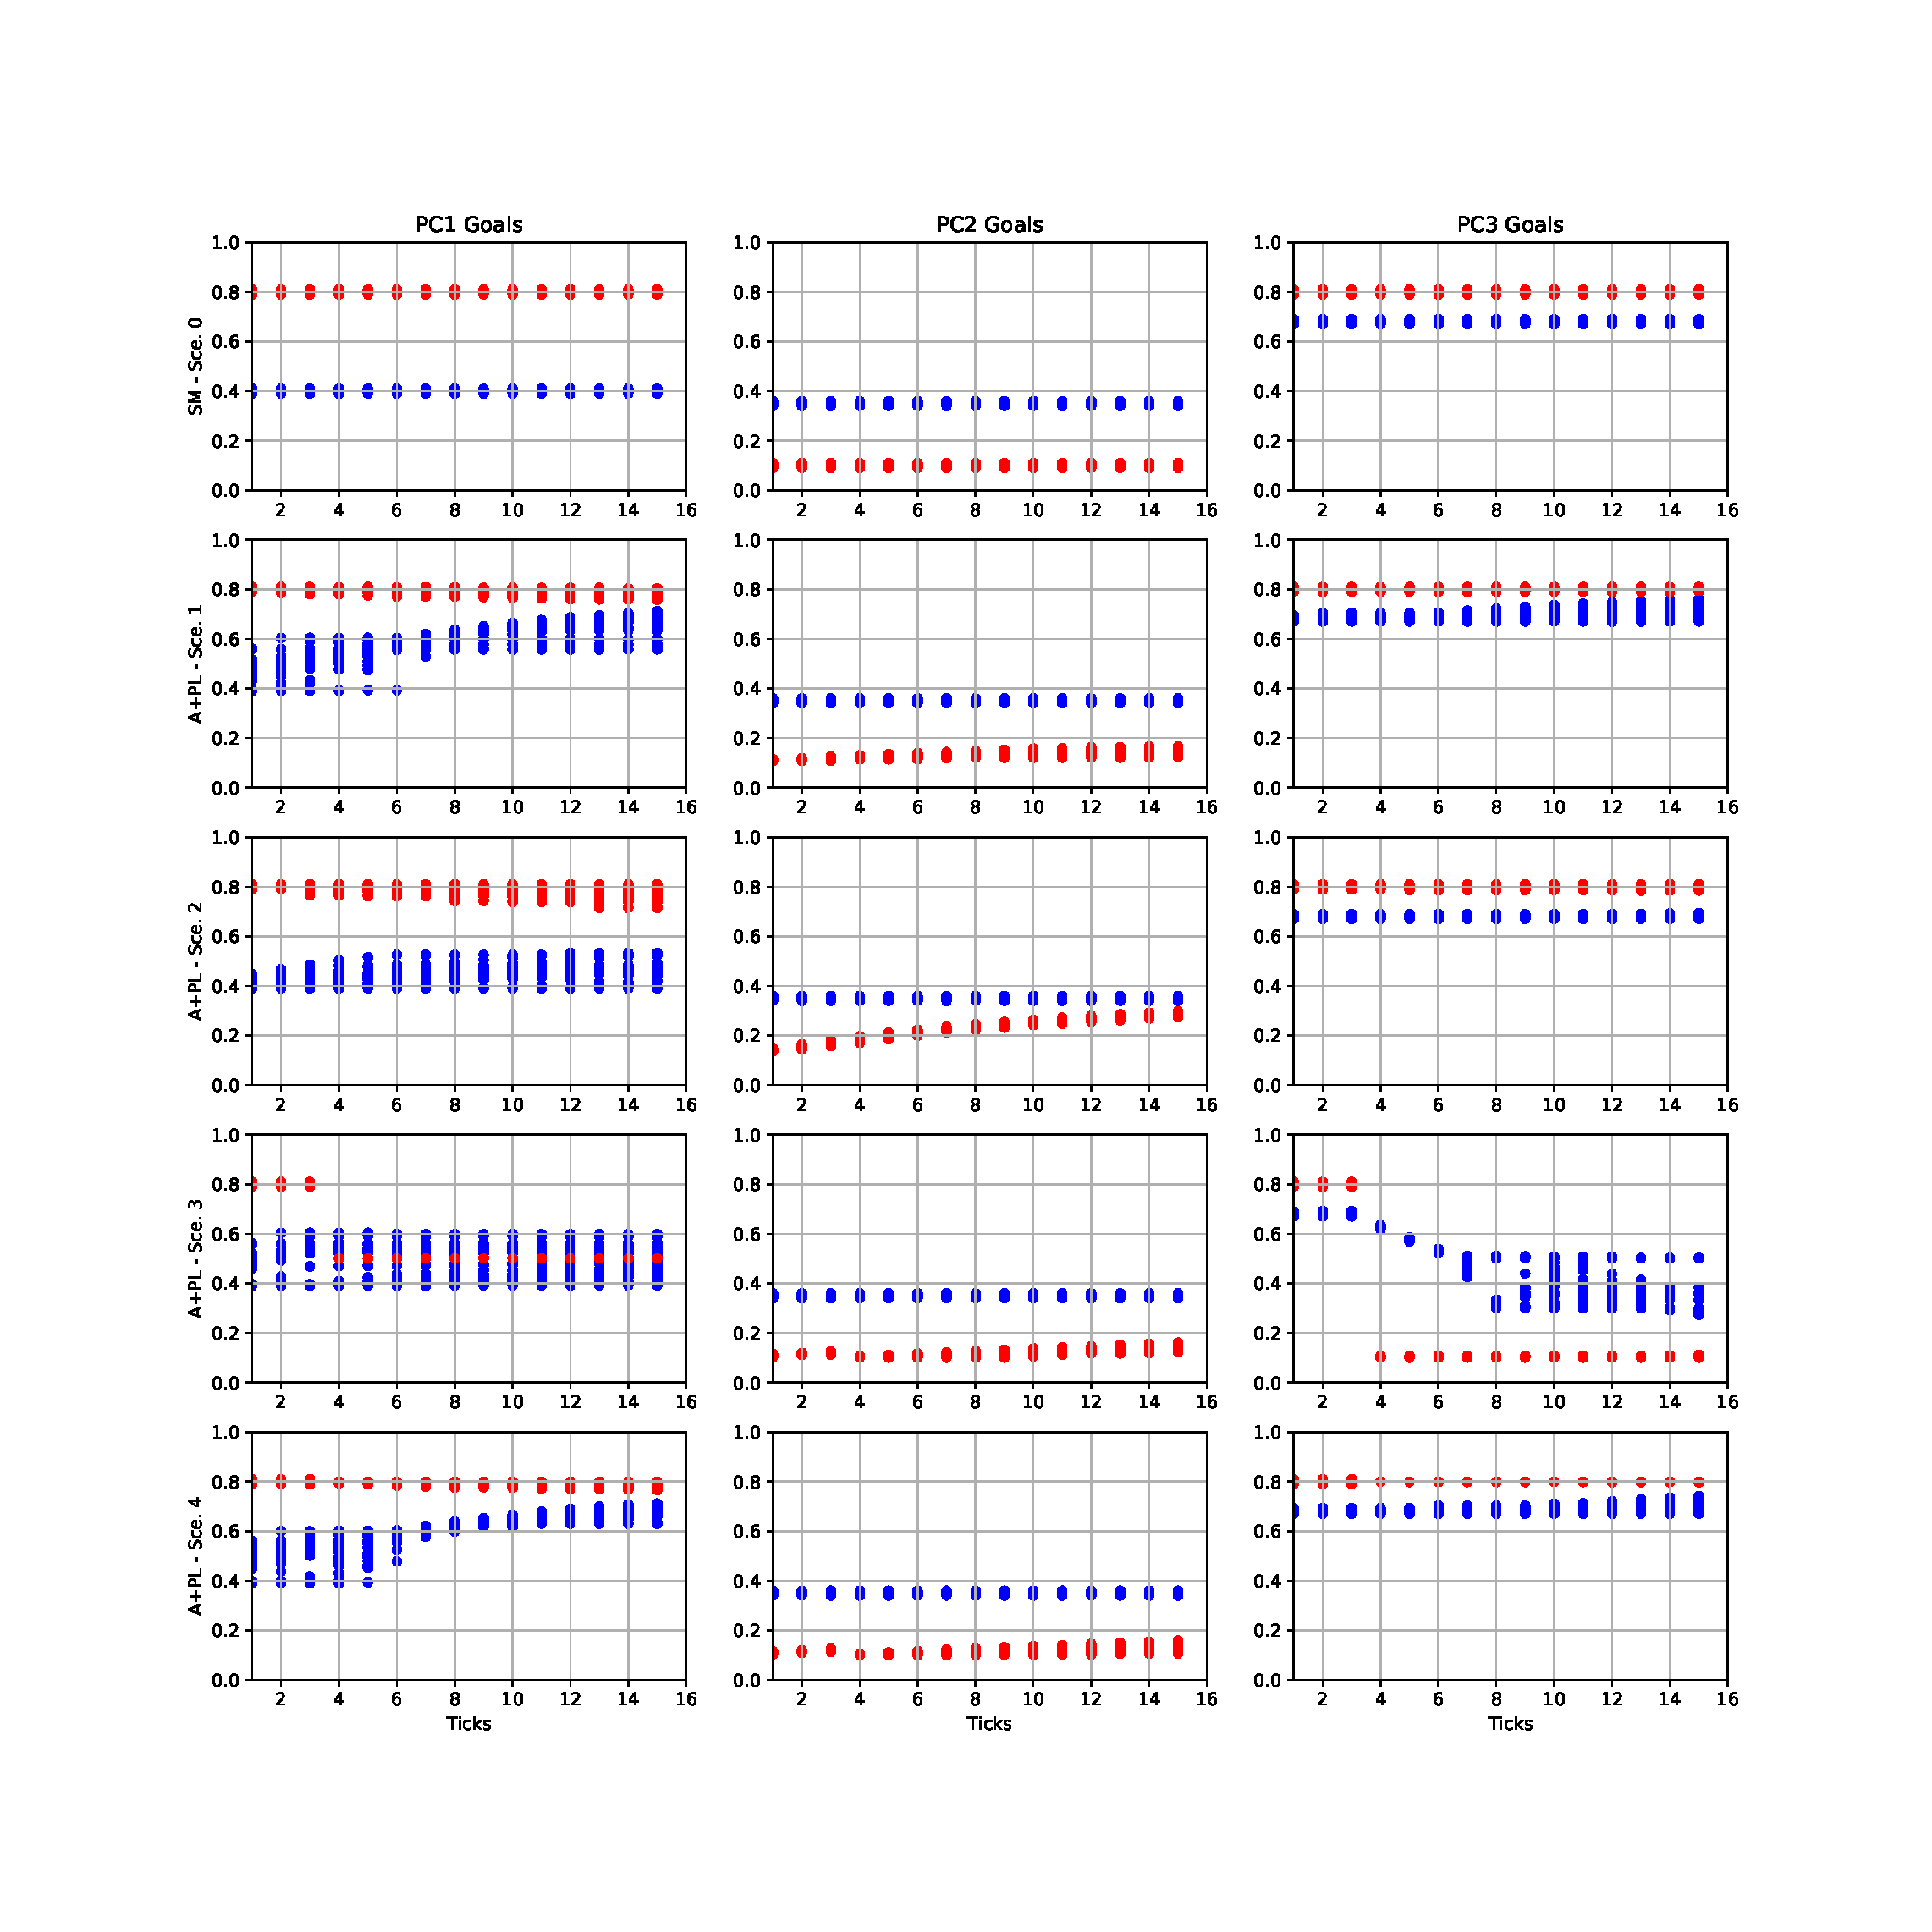
\includegraphics[width = 0.95\linewidth, angle = 0]{figures/PE_PL_PCGoals_+PL}
\caption{Policy core issue goals.}
\label{fig:PE_PL_PCGoals}
\end{figure}

\begin{figure}
\centering
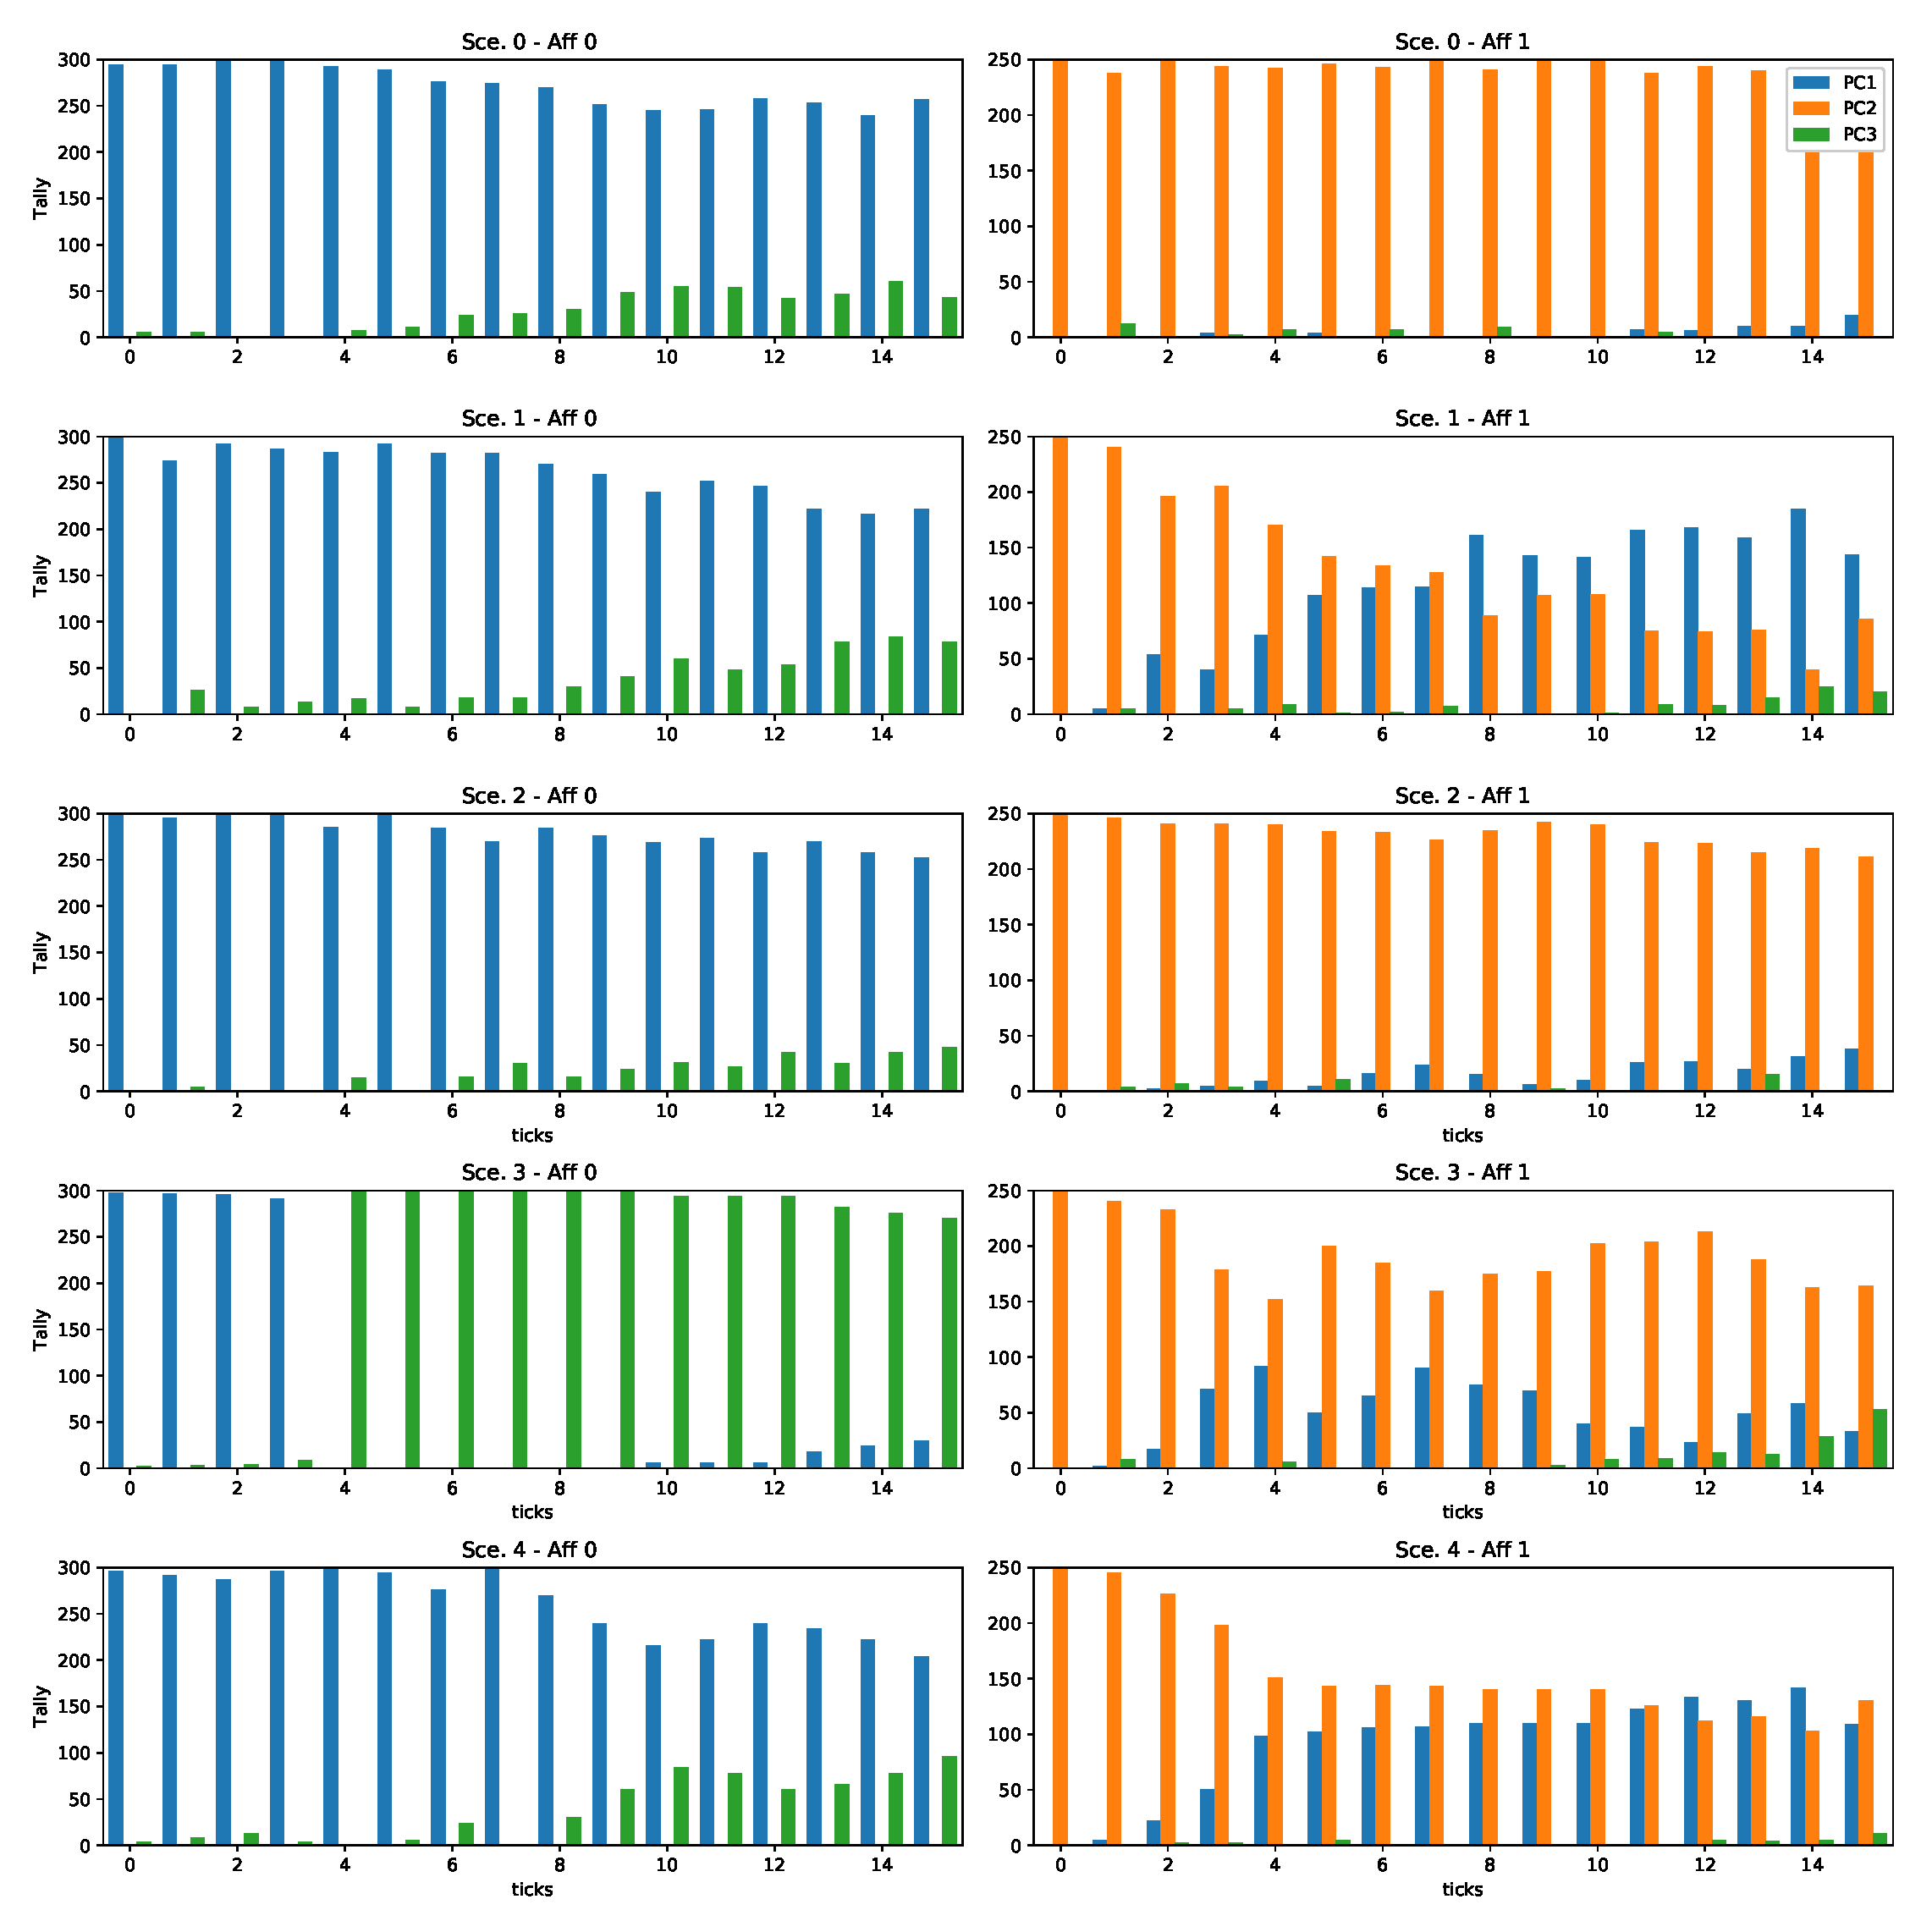
\includegraphics[width = 0.95\linewidth, angle = 0]{figures/PE_PL_PCSelected_+PL}
\caption{Policy core issues selected.}
\label{fig:PE_PL_PCSelected}
\end{figure}

\begin{figure}
\centering
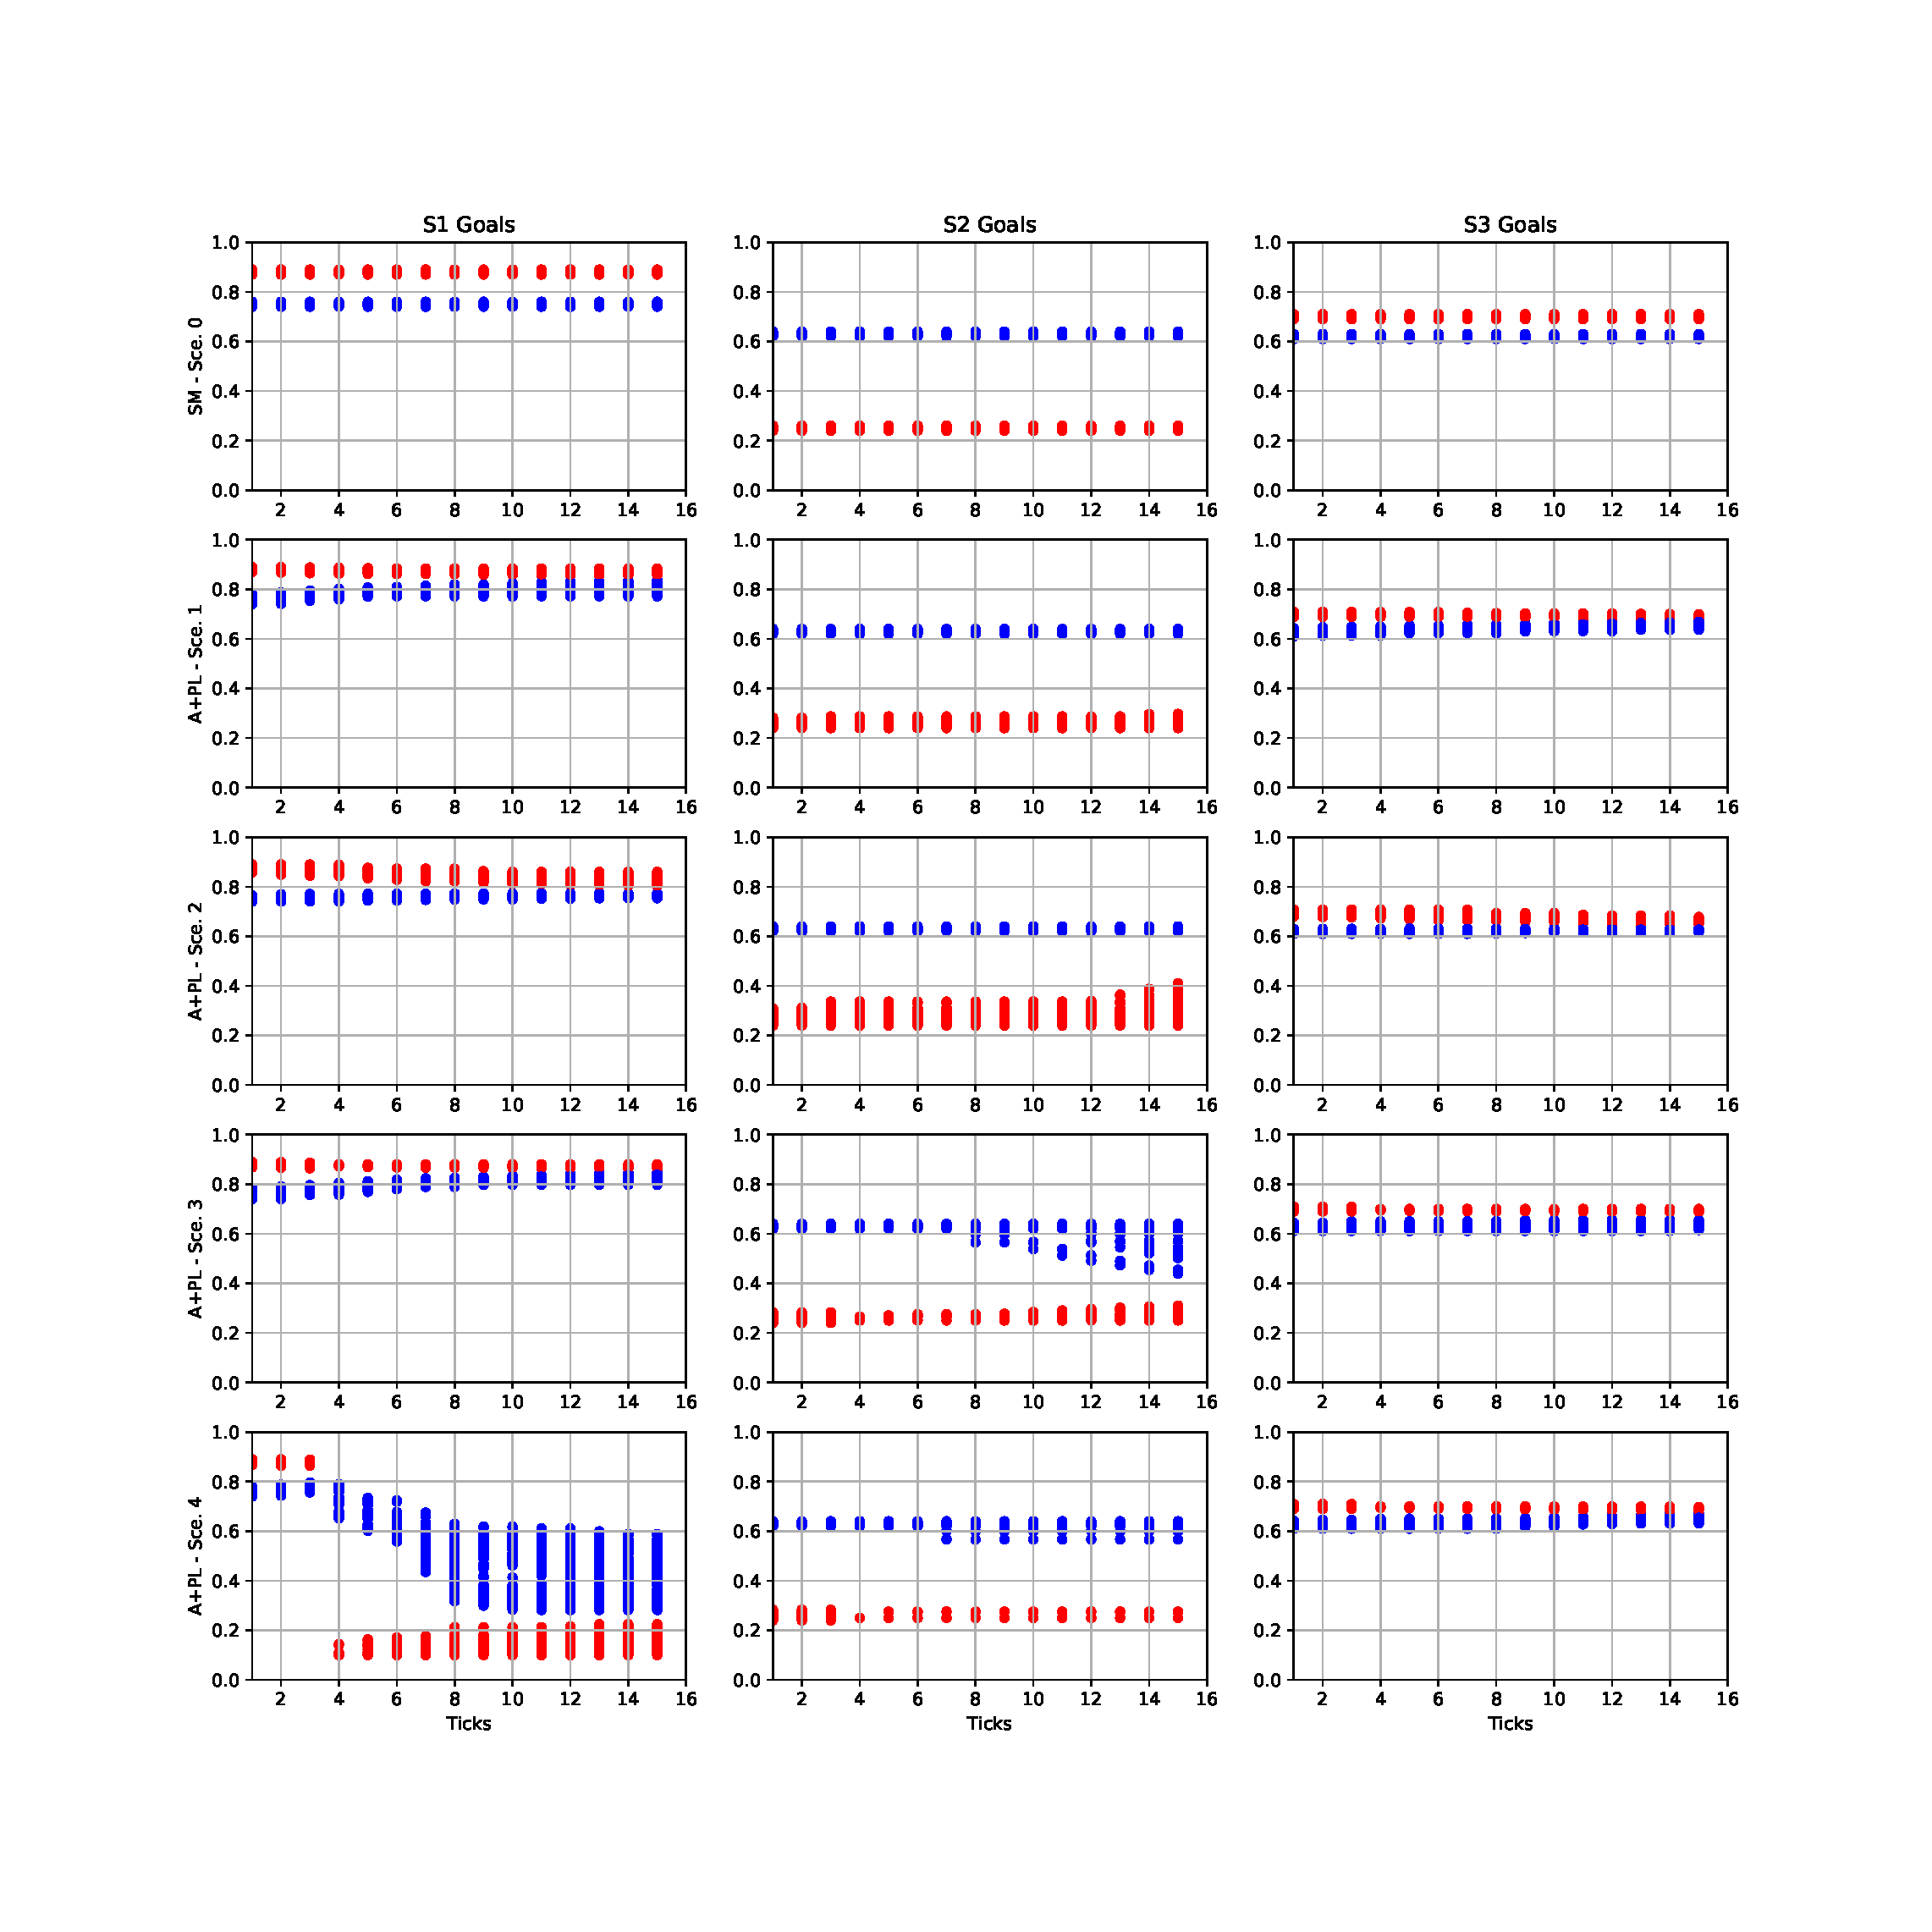
\includegraphics[width = 0.95\linewidth, angle = 0]{figures/PE_PL_SGoals_+PL}
\caption{Secondary issue goals.}
\label{fig:PE_PL_SGoals}
\end{figure}

\begin{figure}
\centering
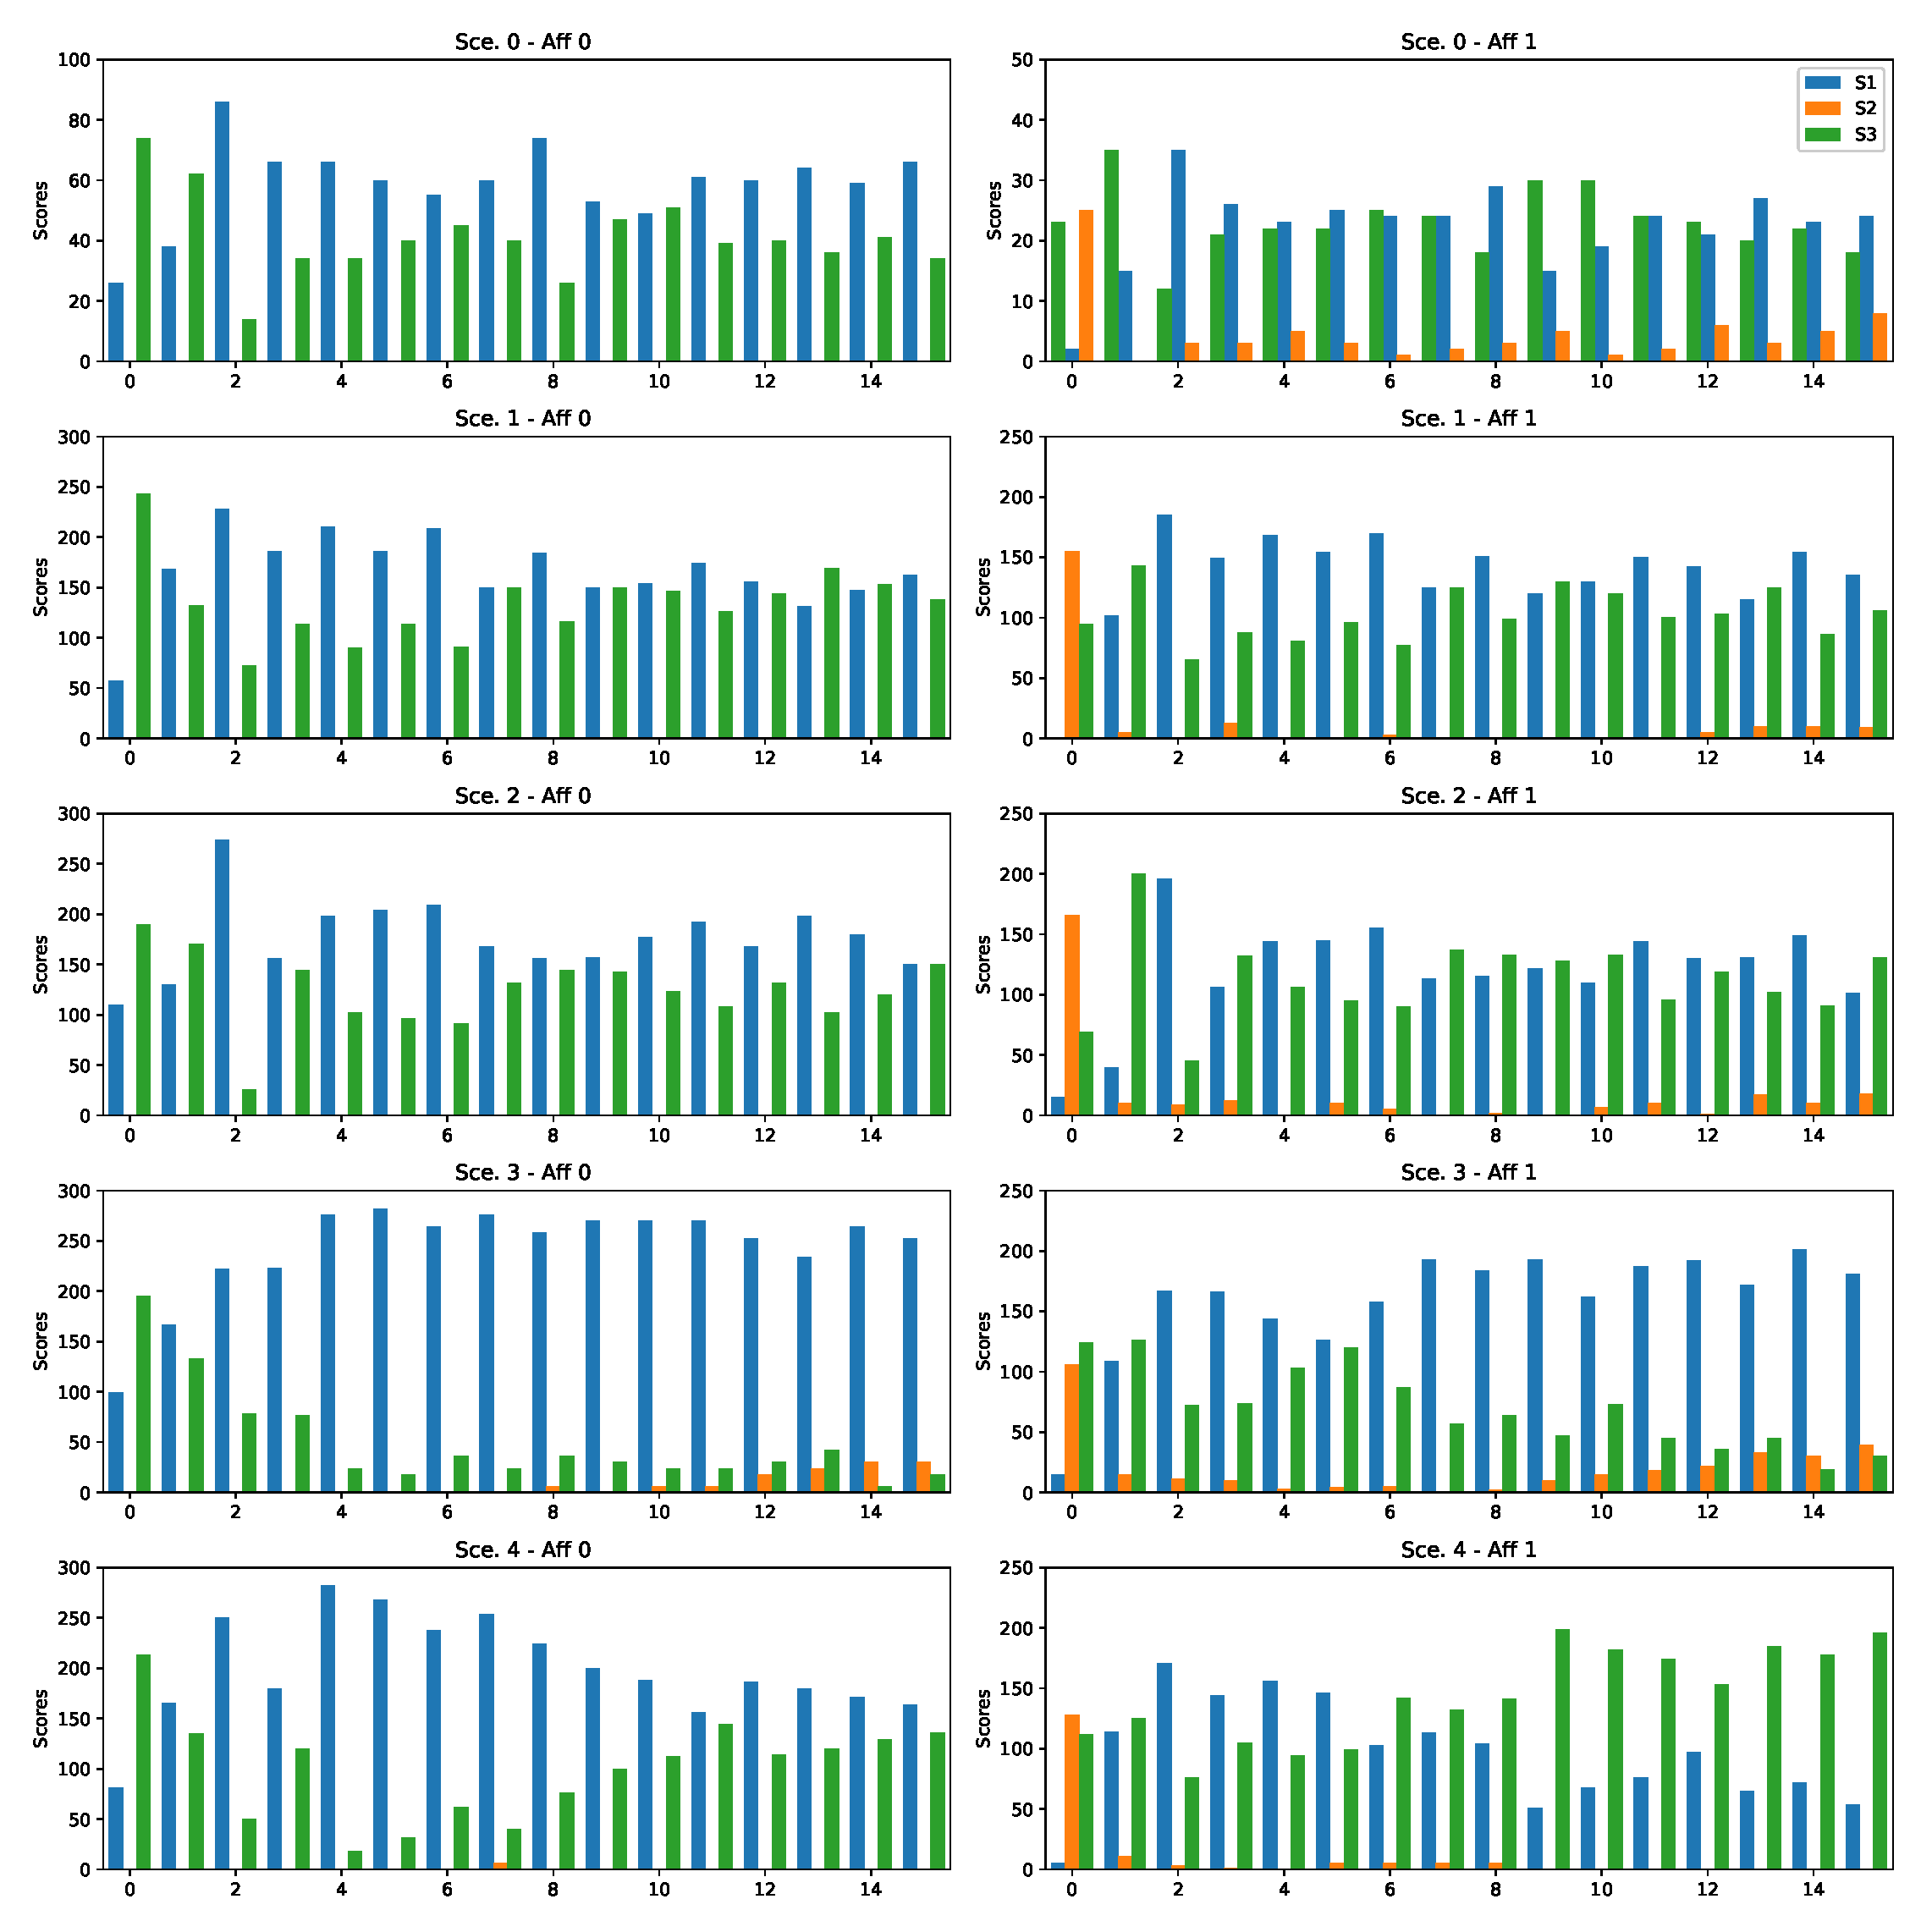
\includegraphics[width = 0.95\linewidth, angle = 0]{figures/PE_PL_SSelected_+PL}
\caption{Secondary issue selected.}
\label{fig:PE_PL_SSelected}
\end{figure}

\begin{figure}
\centering
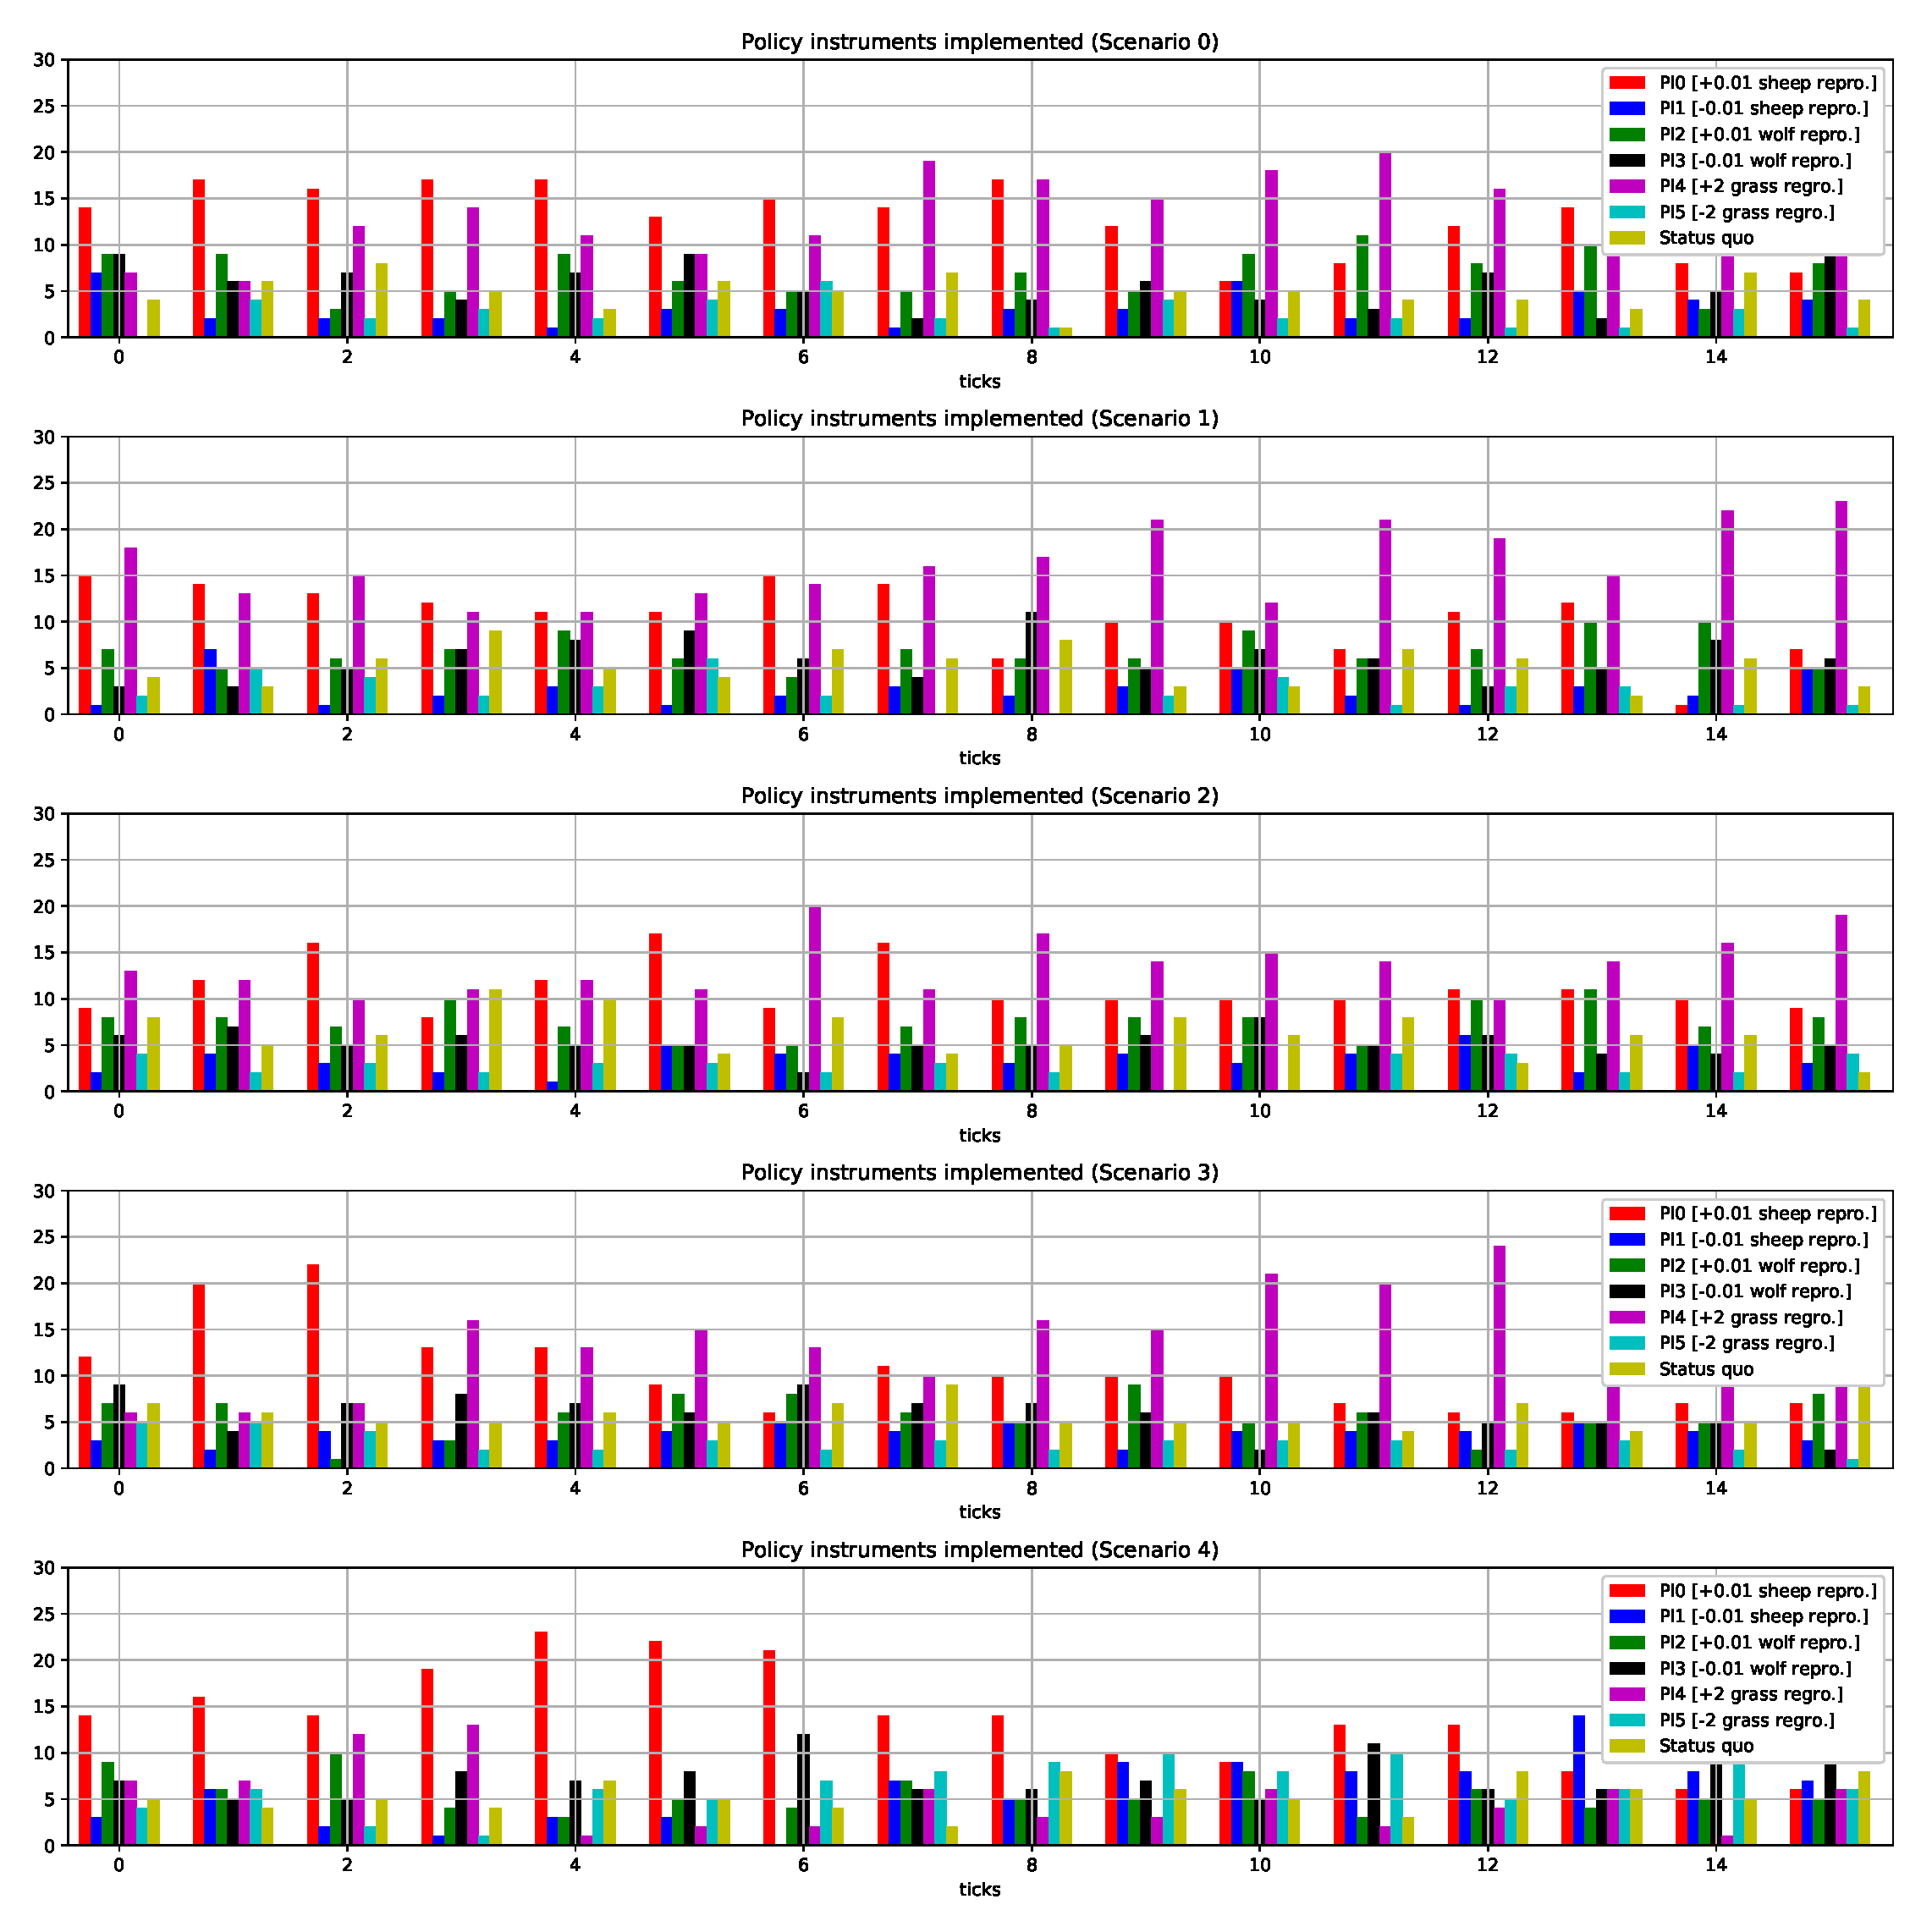
\includegraphics[width = 0.95\linewidth, angle = 0]{figures/PE_PI_selection_+PL}
\caption{Policy instruments selected.}
\label{fig:PE_PI_selection}
\end{figure}

\begin{figure}
\centering
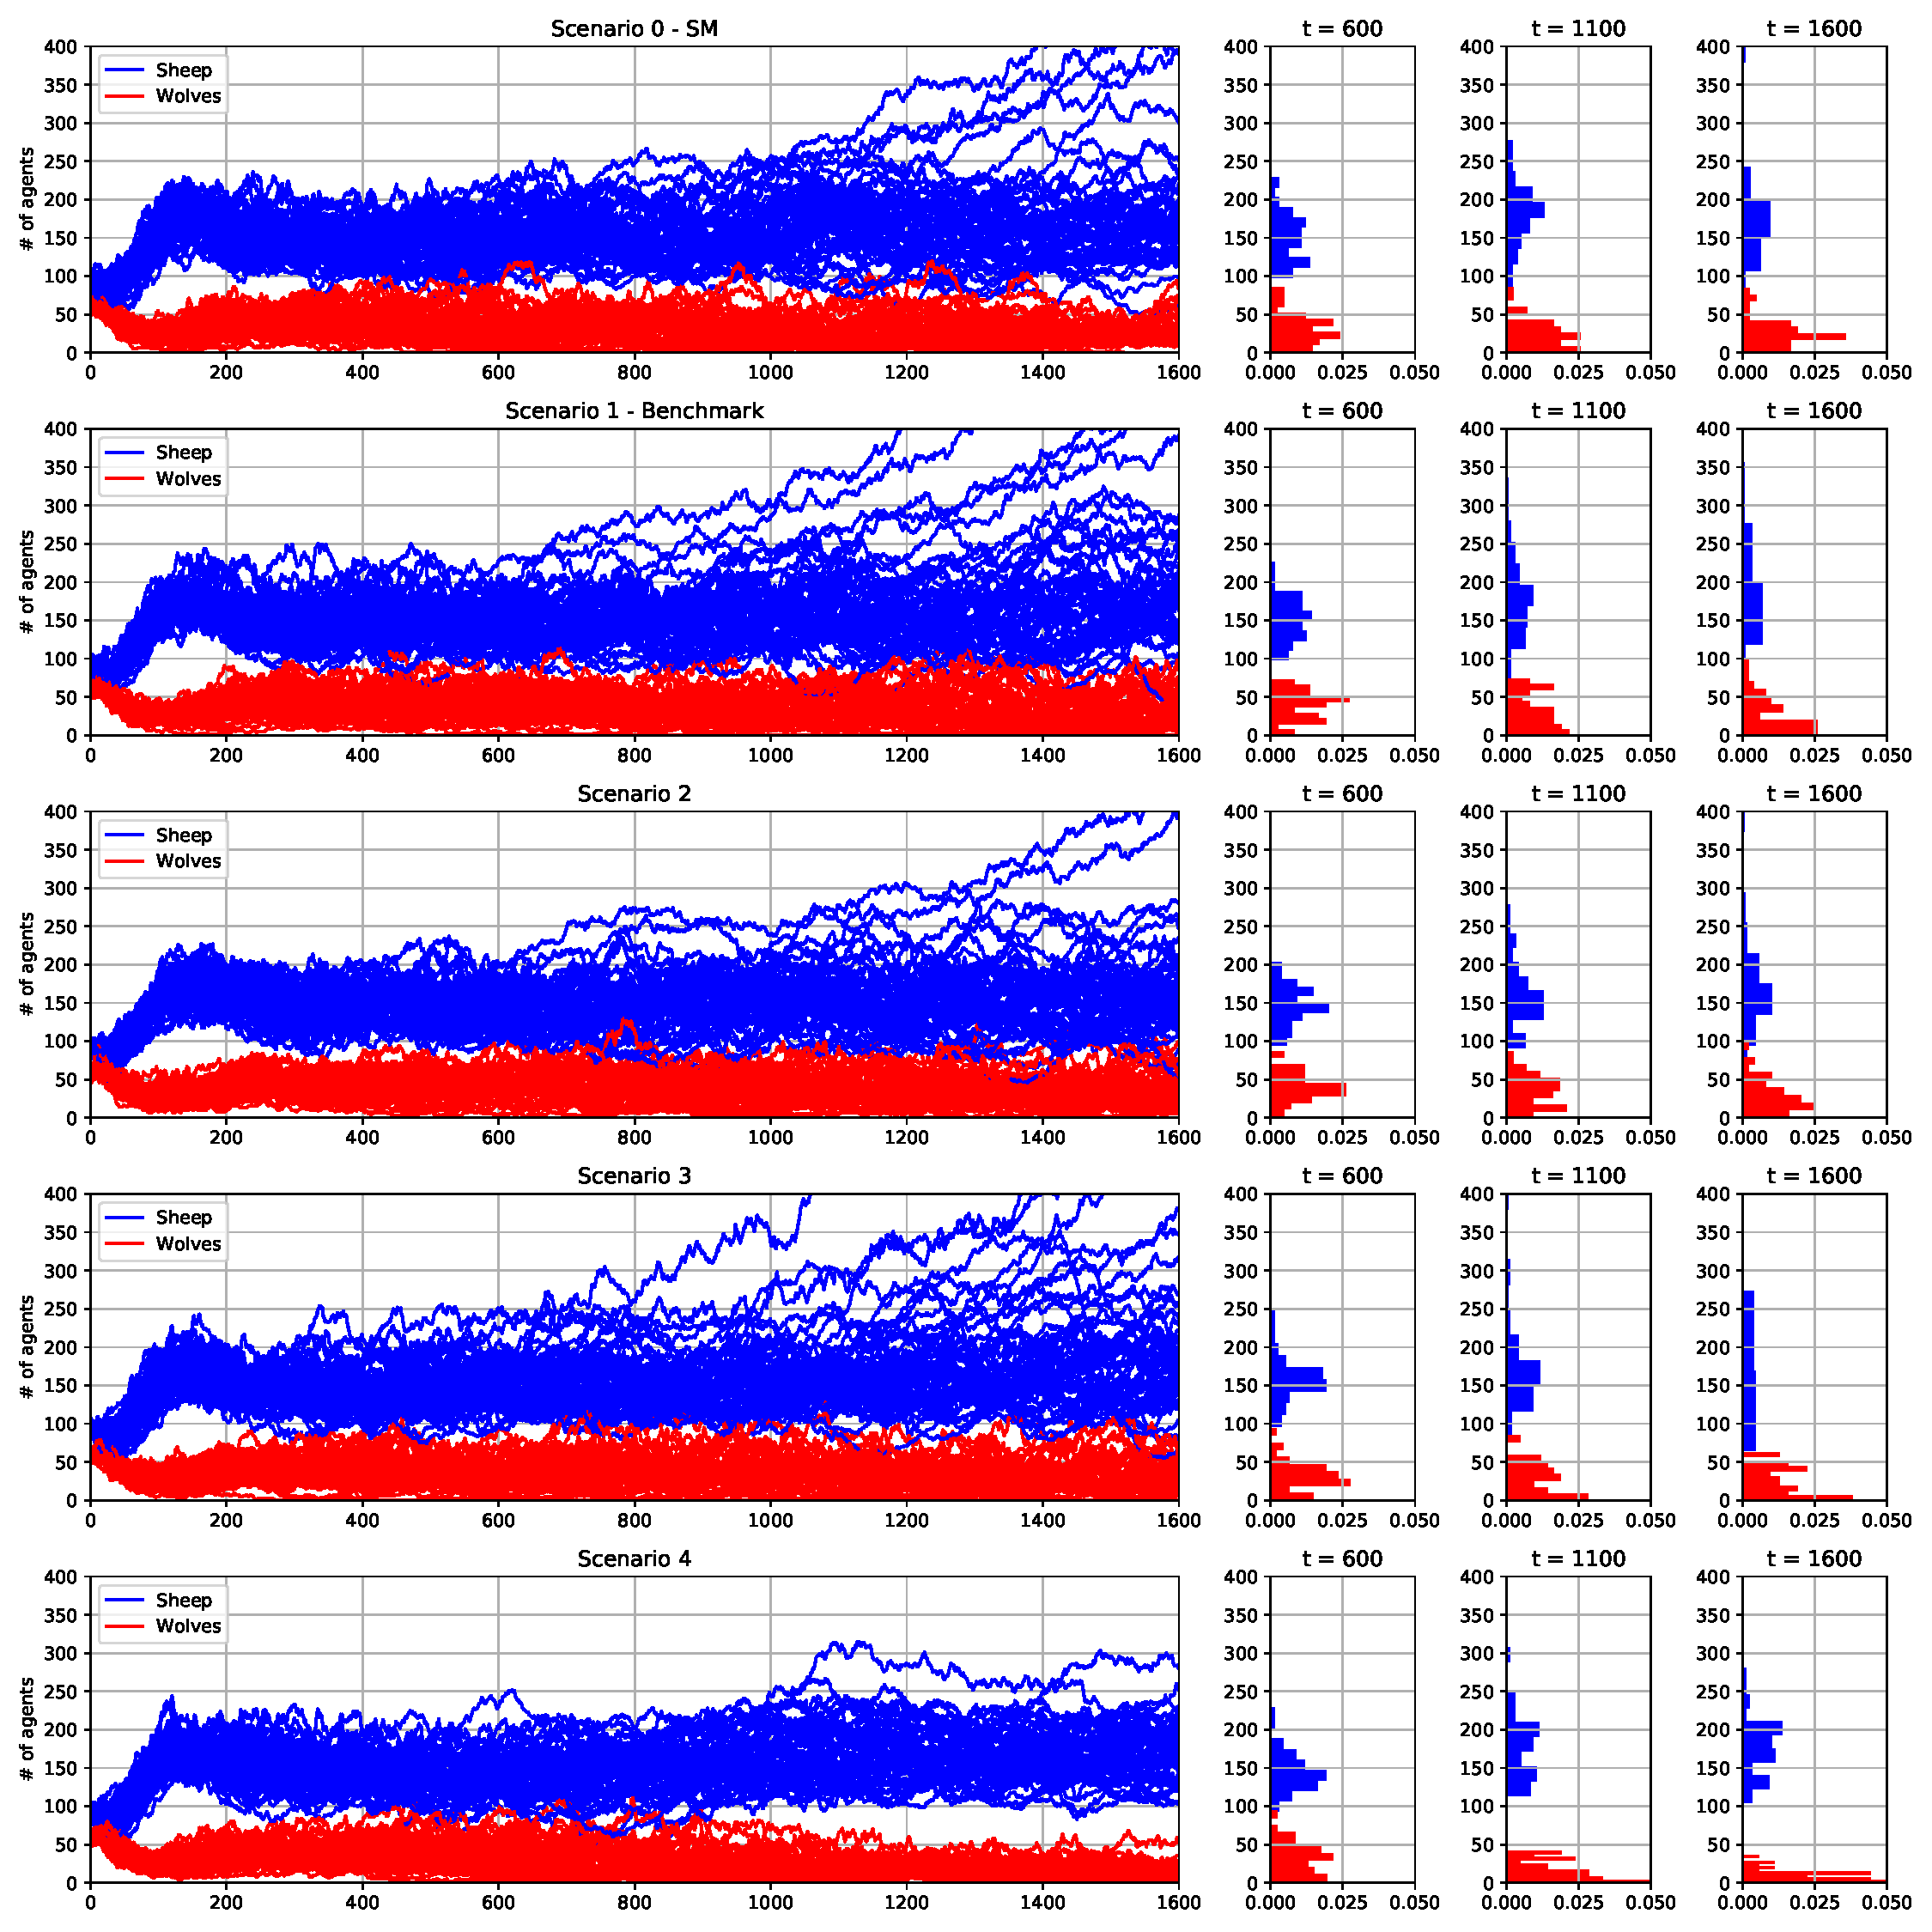
\includegraphics[width = 0.95\linewidth, angle = 0]{figures/Predation_Q1_popsWolfSheep_+PL}
\caption{Predation model results - wolf and sheep.}
\label{fig:Predation_Q1_popsWolfSheep}
\end{figure}

\begin{figure}
\centering
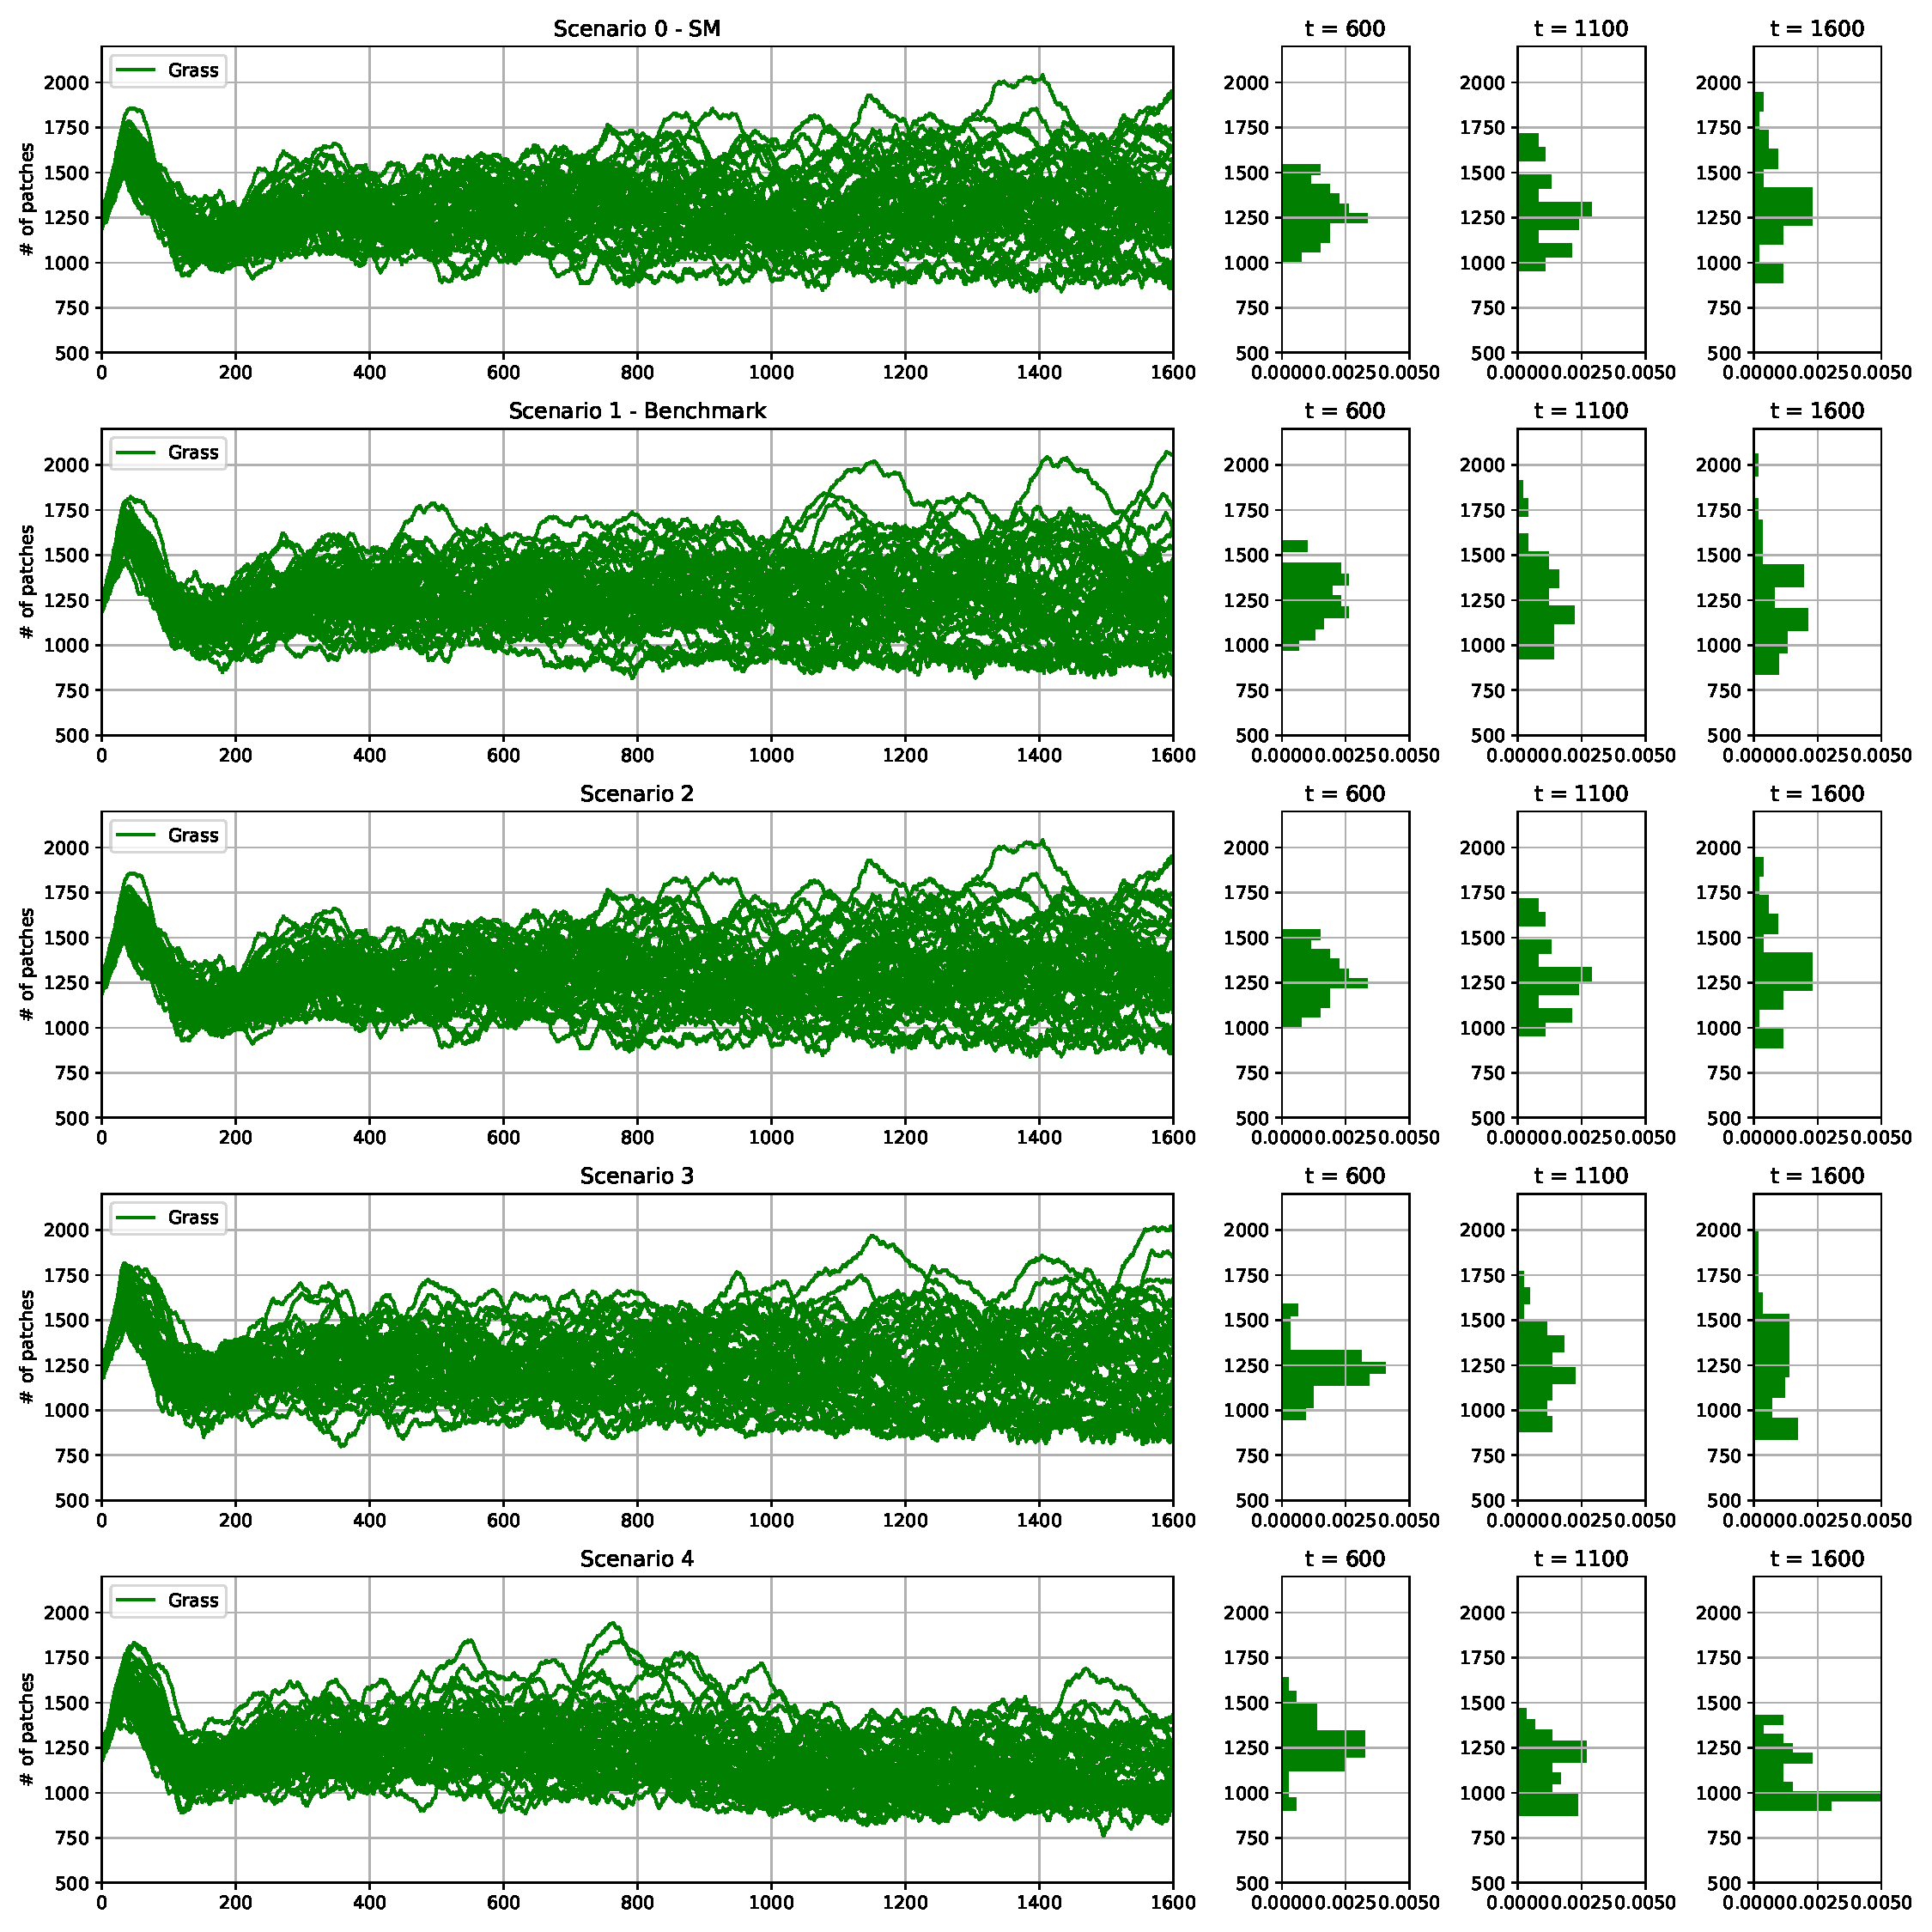
\includegraphics[width = 0.95\linewidth, angle = 0]{figures/Predation_Q1_popsGrass_+PL}
\caption{Predation model results - grass.}
\label{fig:Predation_Q1_popsGrass}
\end{figure}

\begin{figure}
\centering
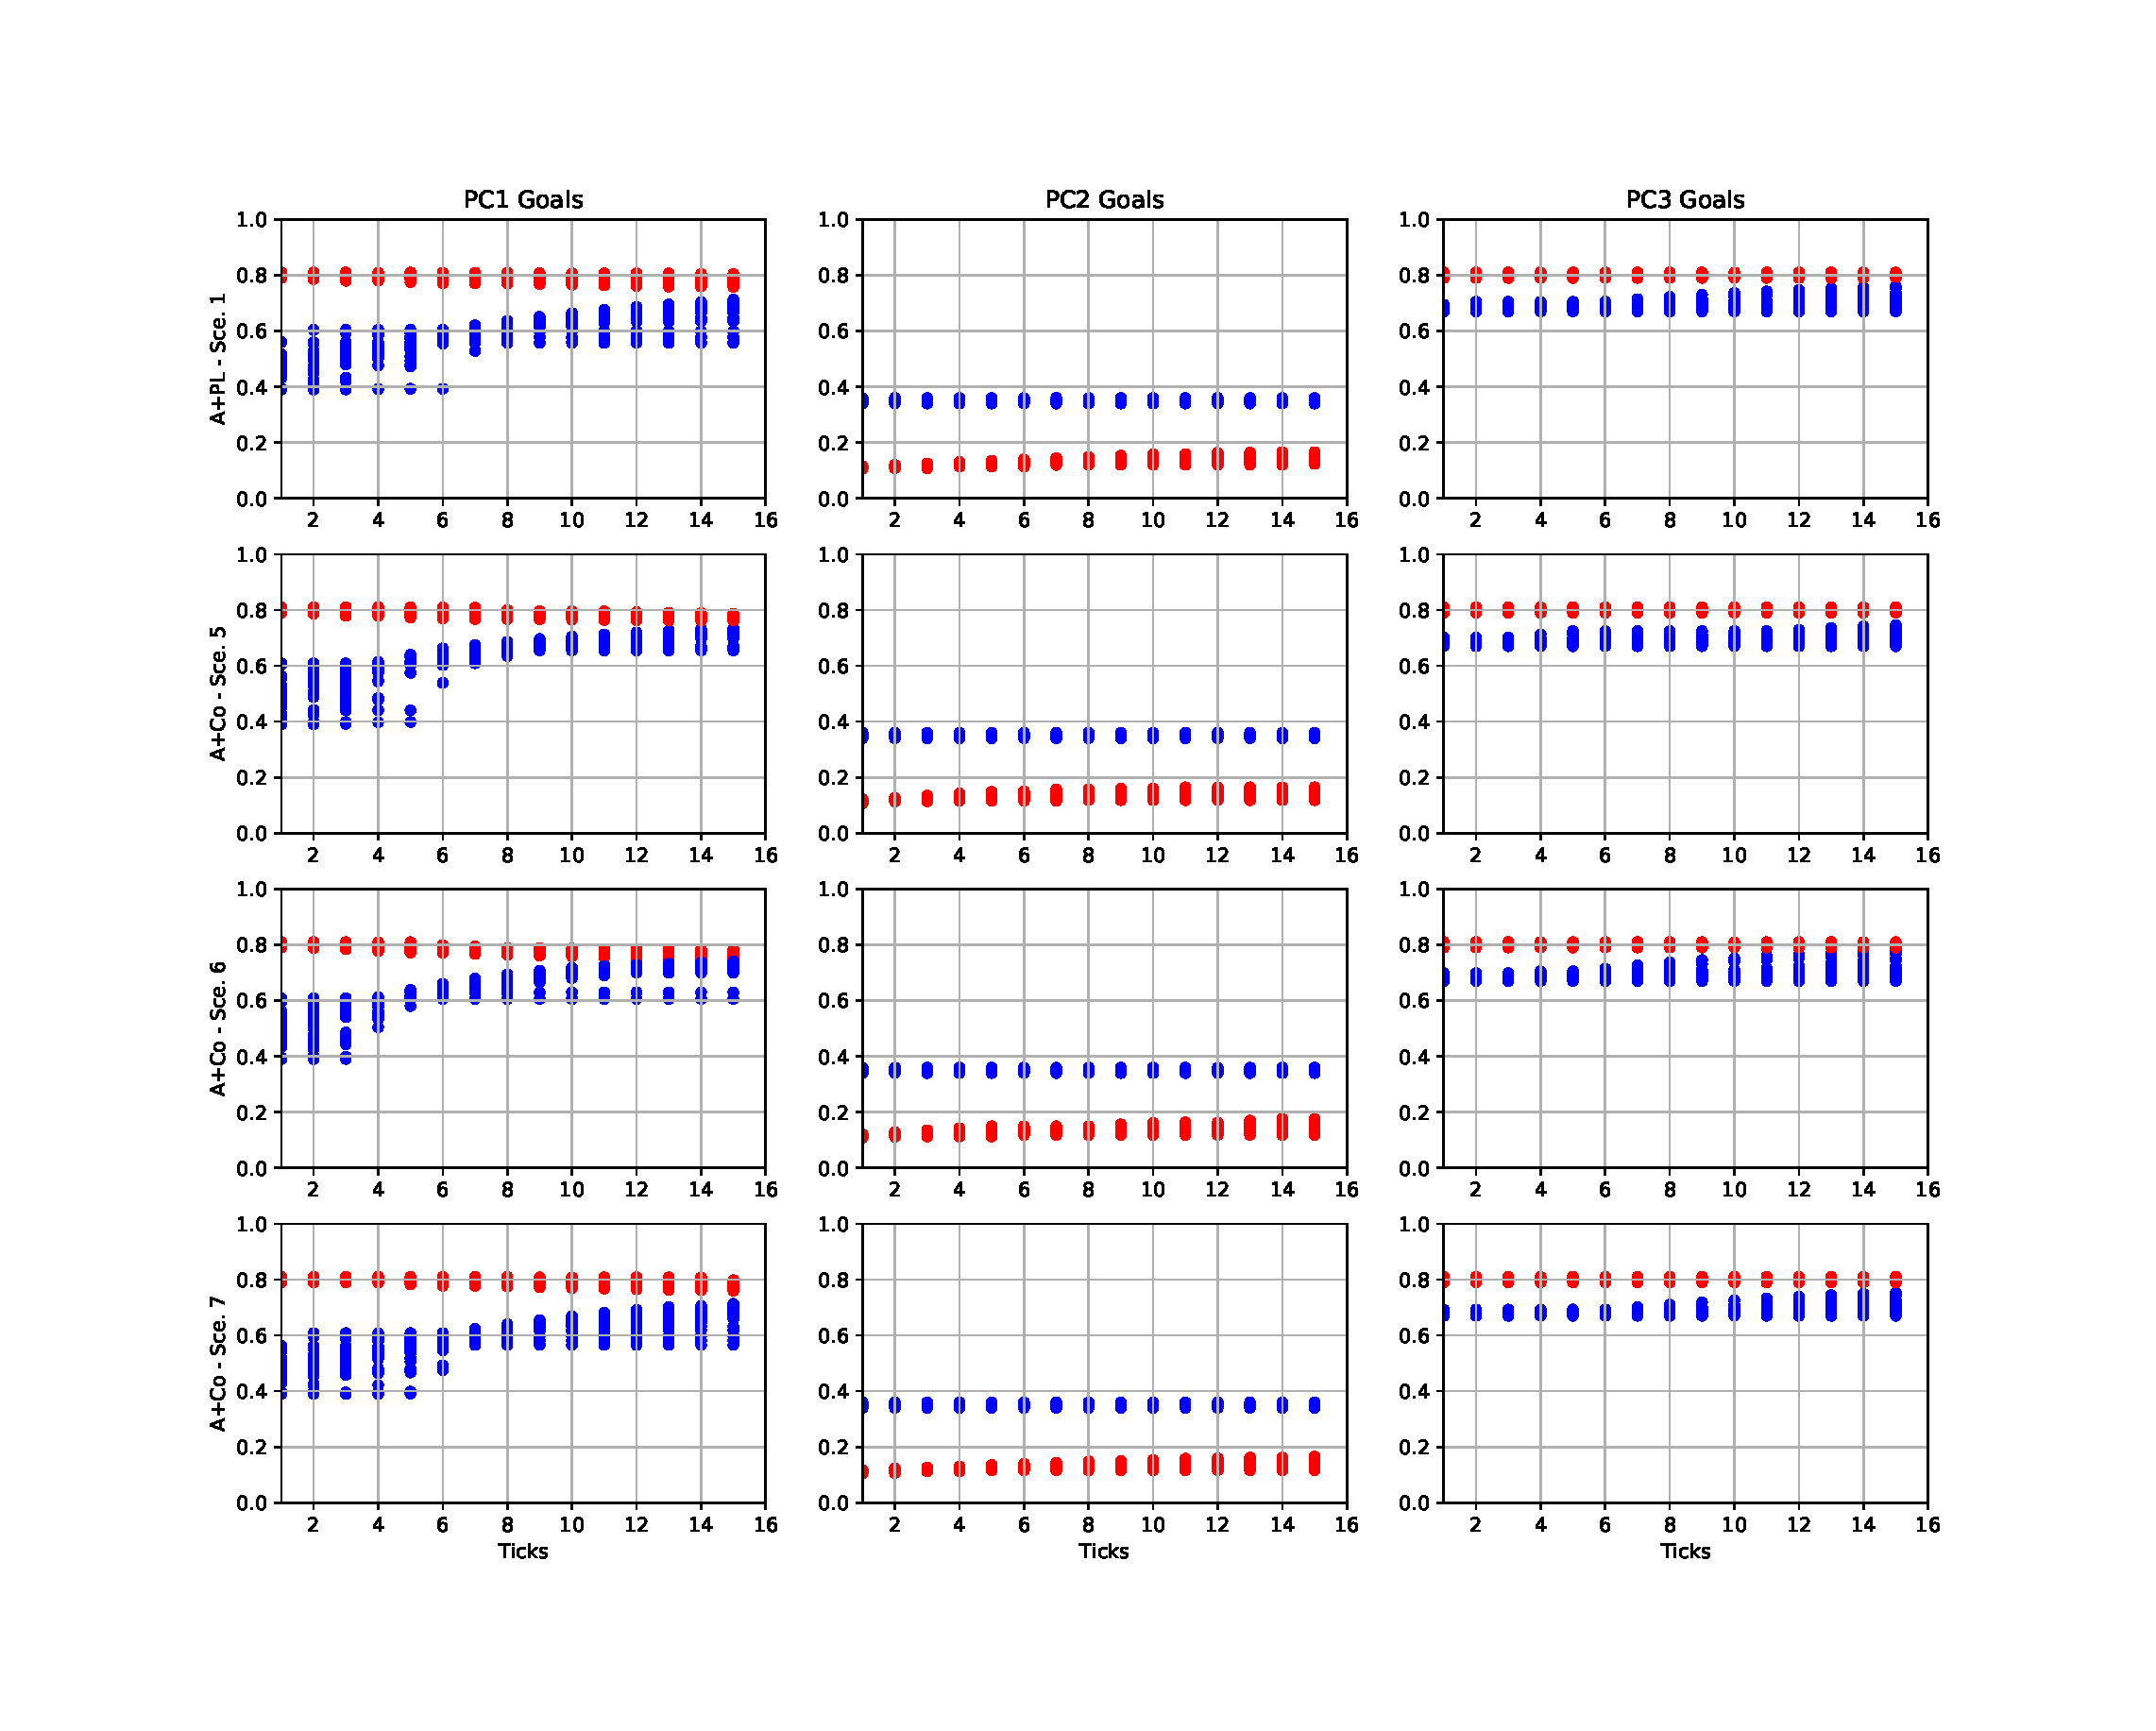
\includegraphics[width = 0.95\linewidth, angle = 0]{figures/PE_PL_PCGoals_+Co}
\caption{Policy core issue goals.}
\label{fig:PE_PL_PCGoals}
\end{figure}

\begin{figure}
\centering
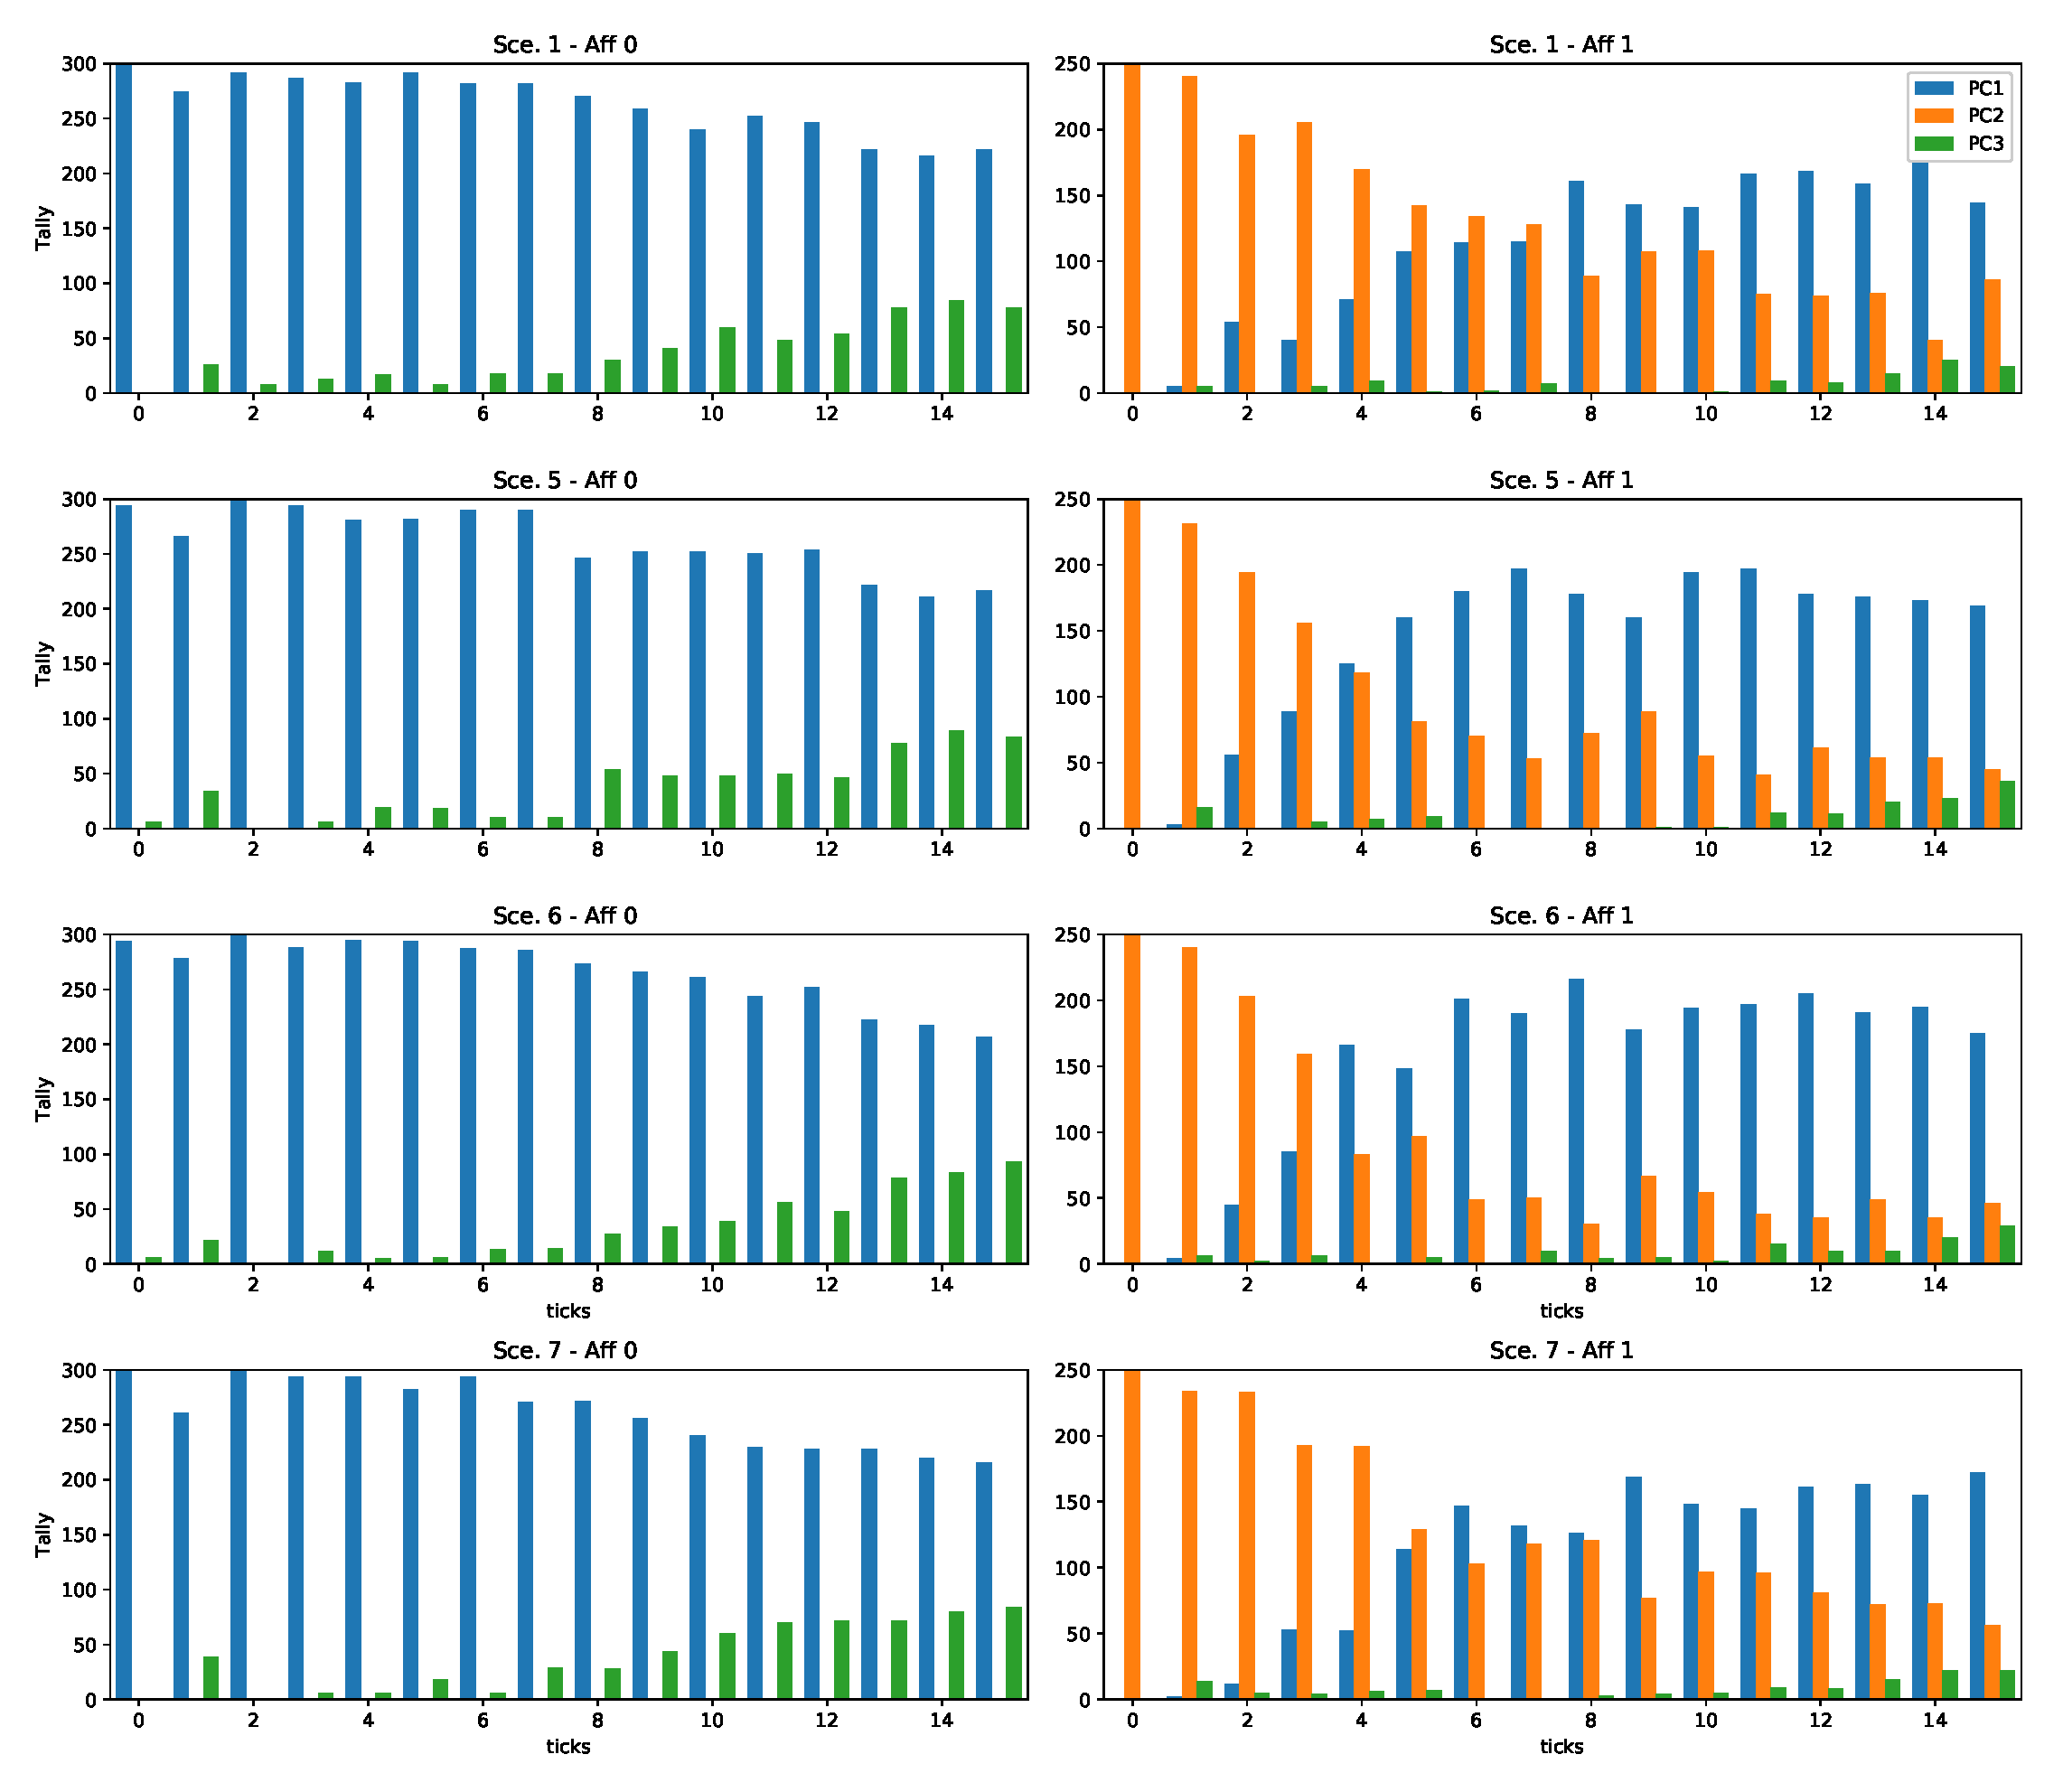
\includegraphics[width = 0.95\linewidth, angle = 0]{figures/PE_PL_PCSelected_+Co}
\caption{Policy core issues selected.}
\label{fig:PE_PL_PCSelected}
\end{figure}

\begin{figure}
\centering
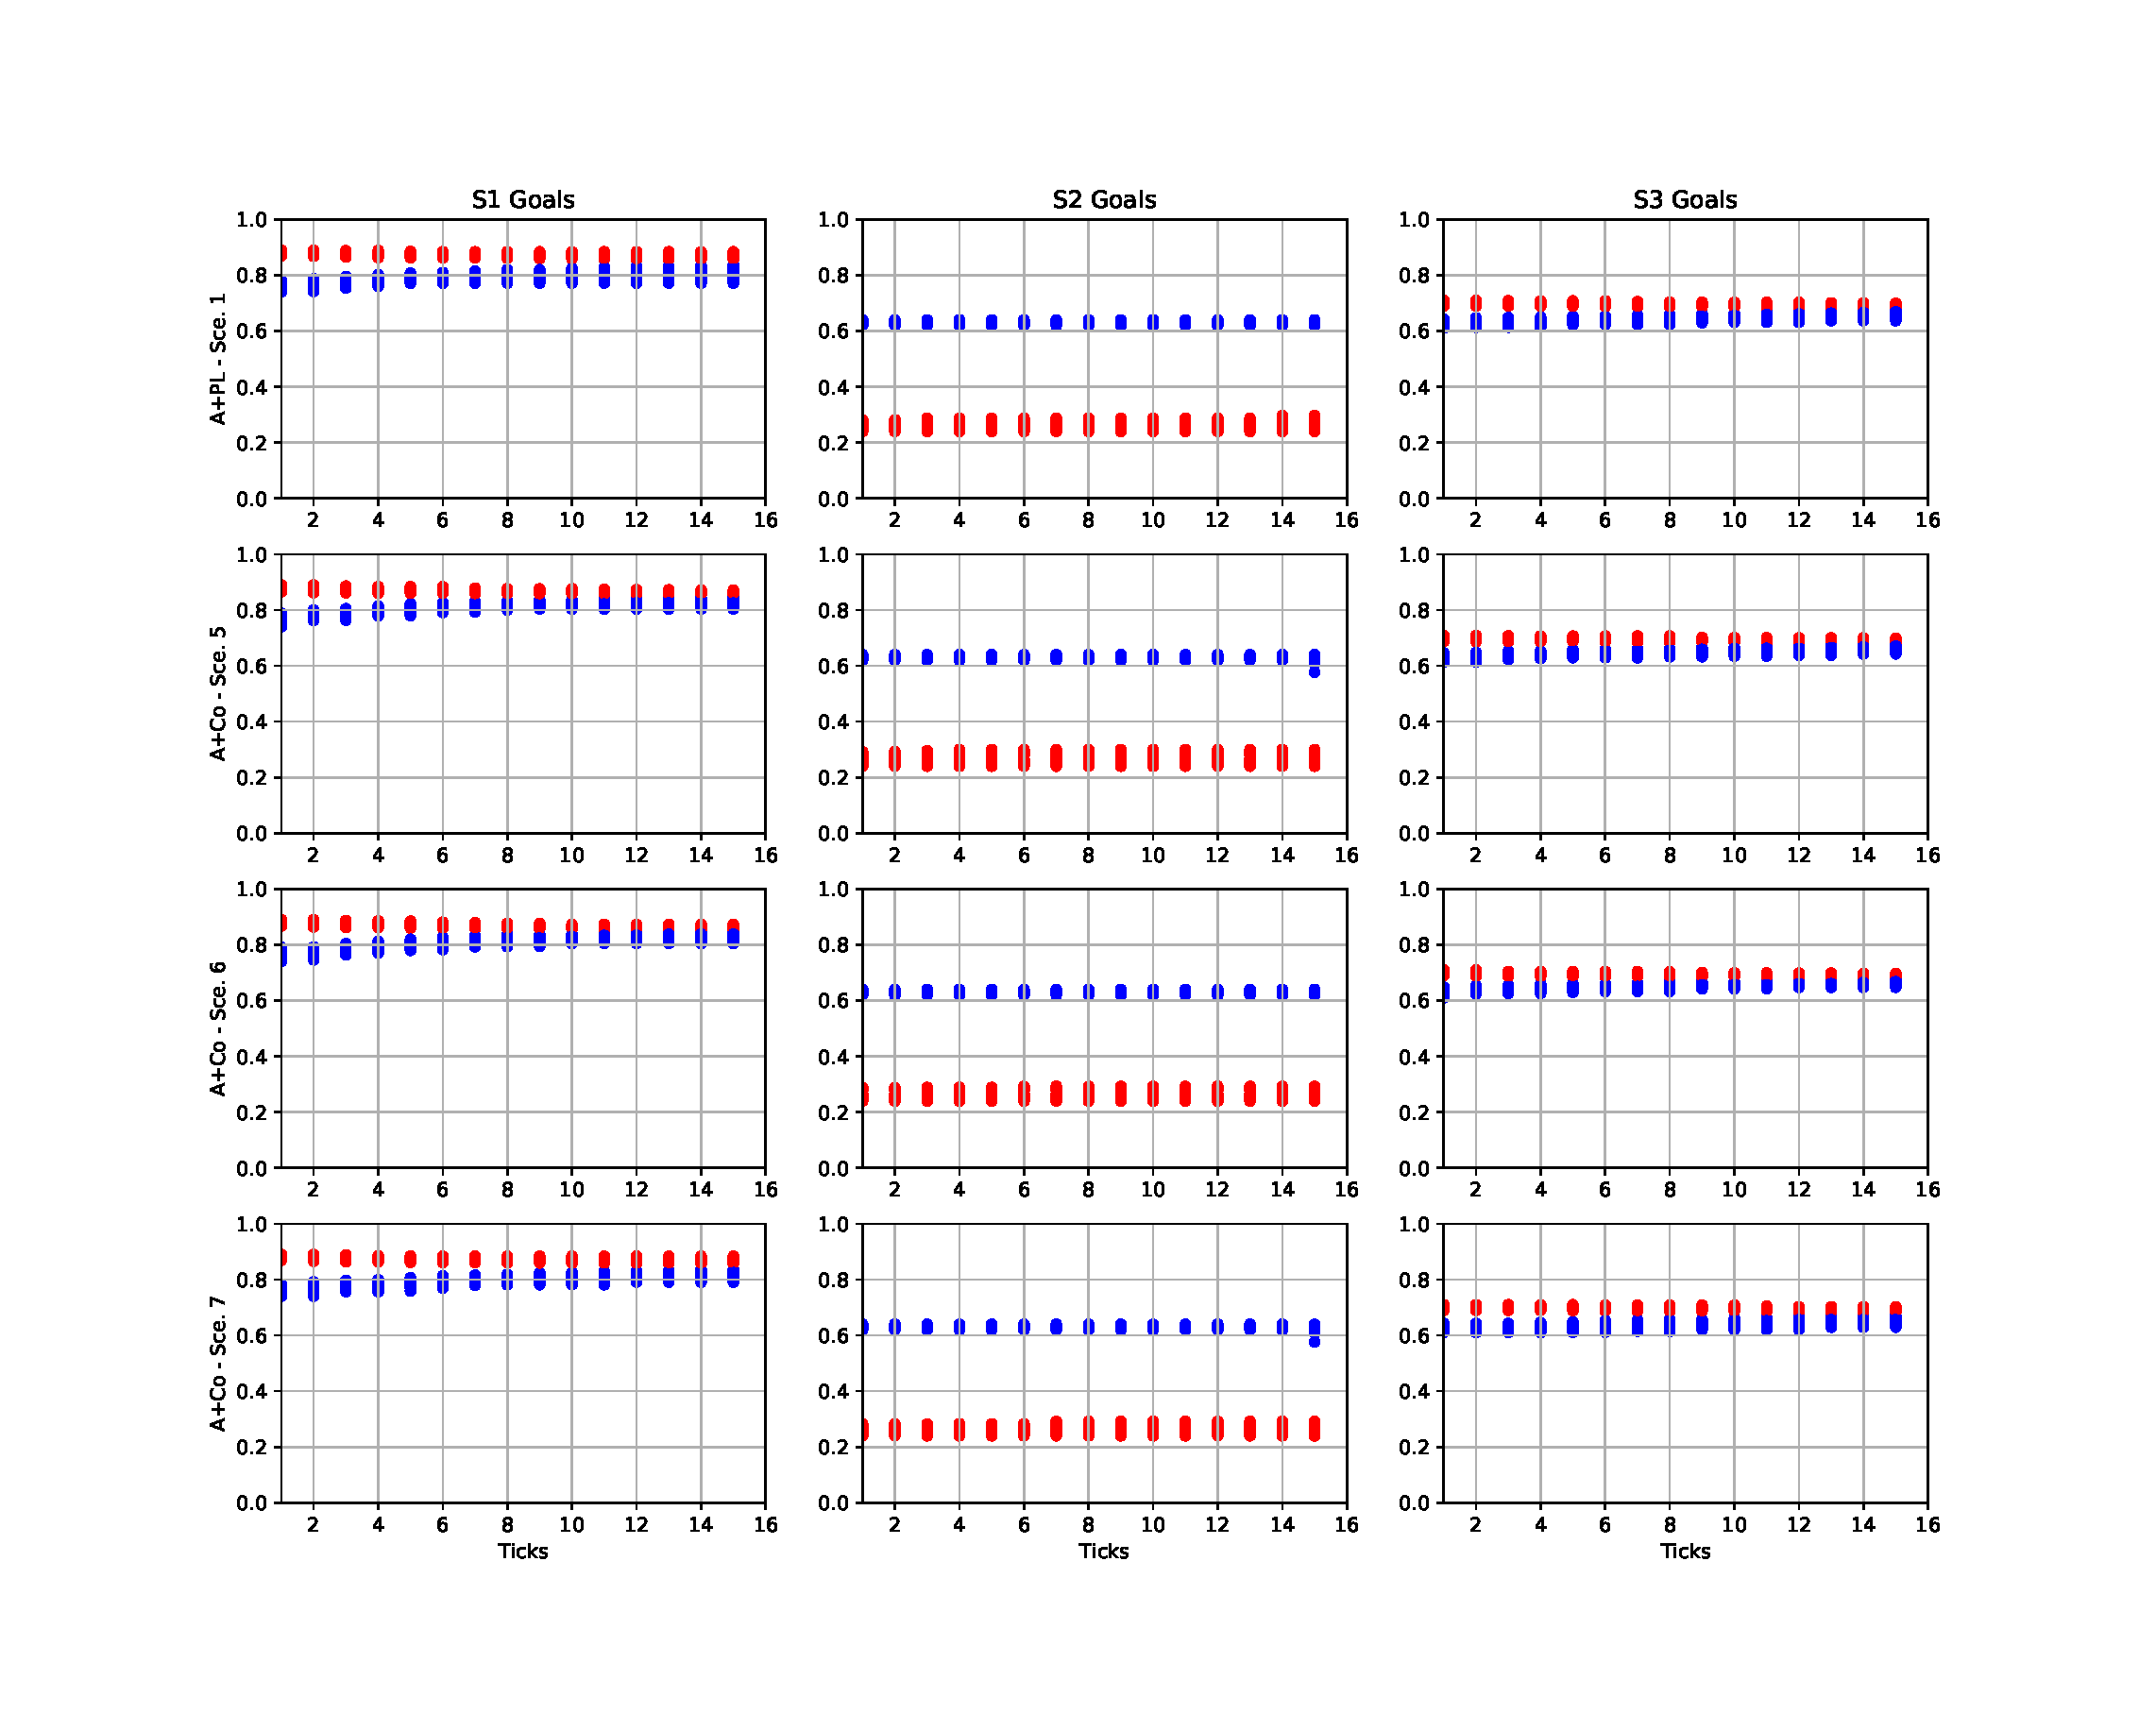
\includegraphics[width = 0.95\linewidth, angle = 0]{figures/PE_PL_SGoals_+Co}
\caption{Secondary issue goals.}
\label{fig:PE_PL_SGoals}
\end{figure}

\begin{figure}
\centering
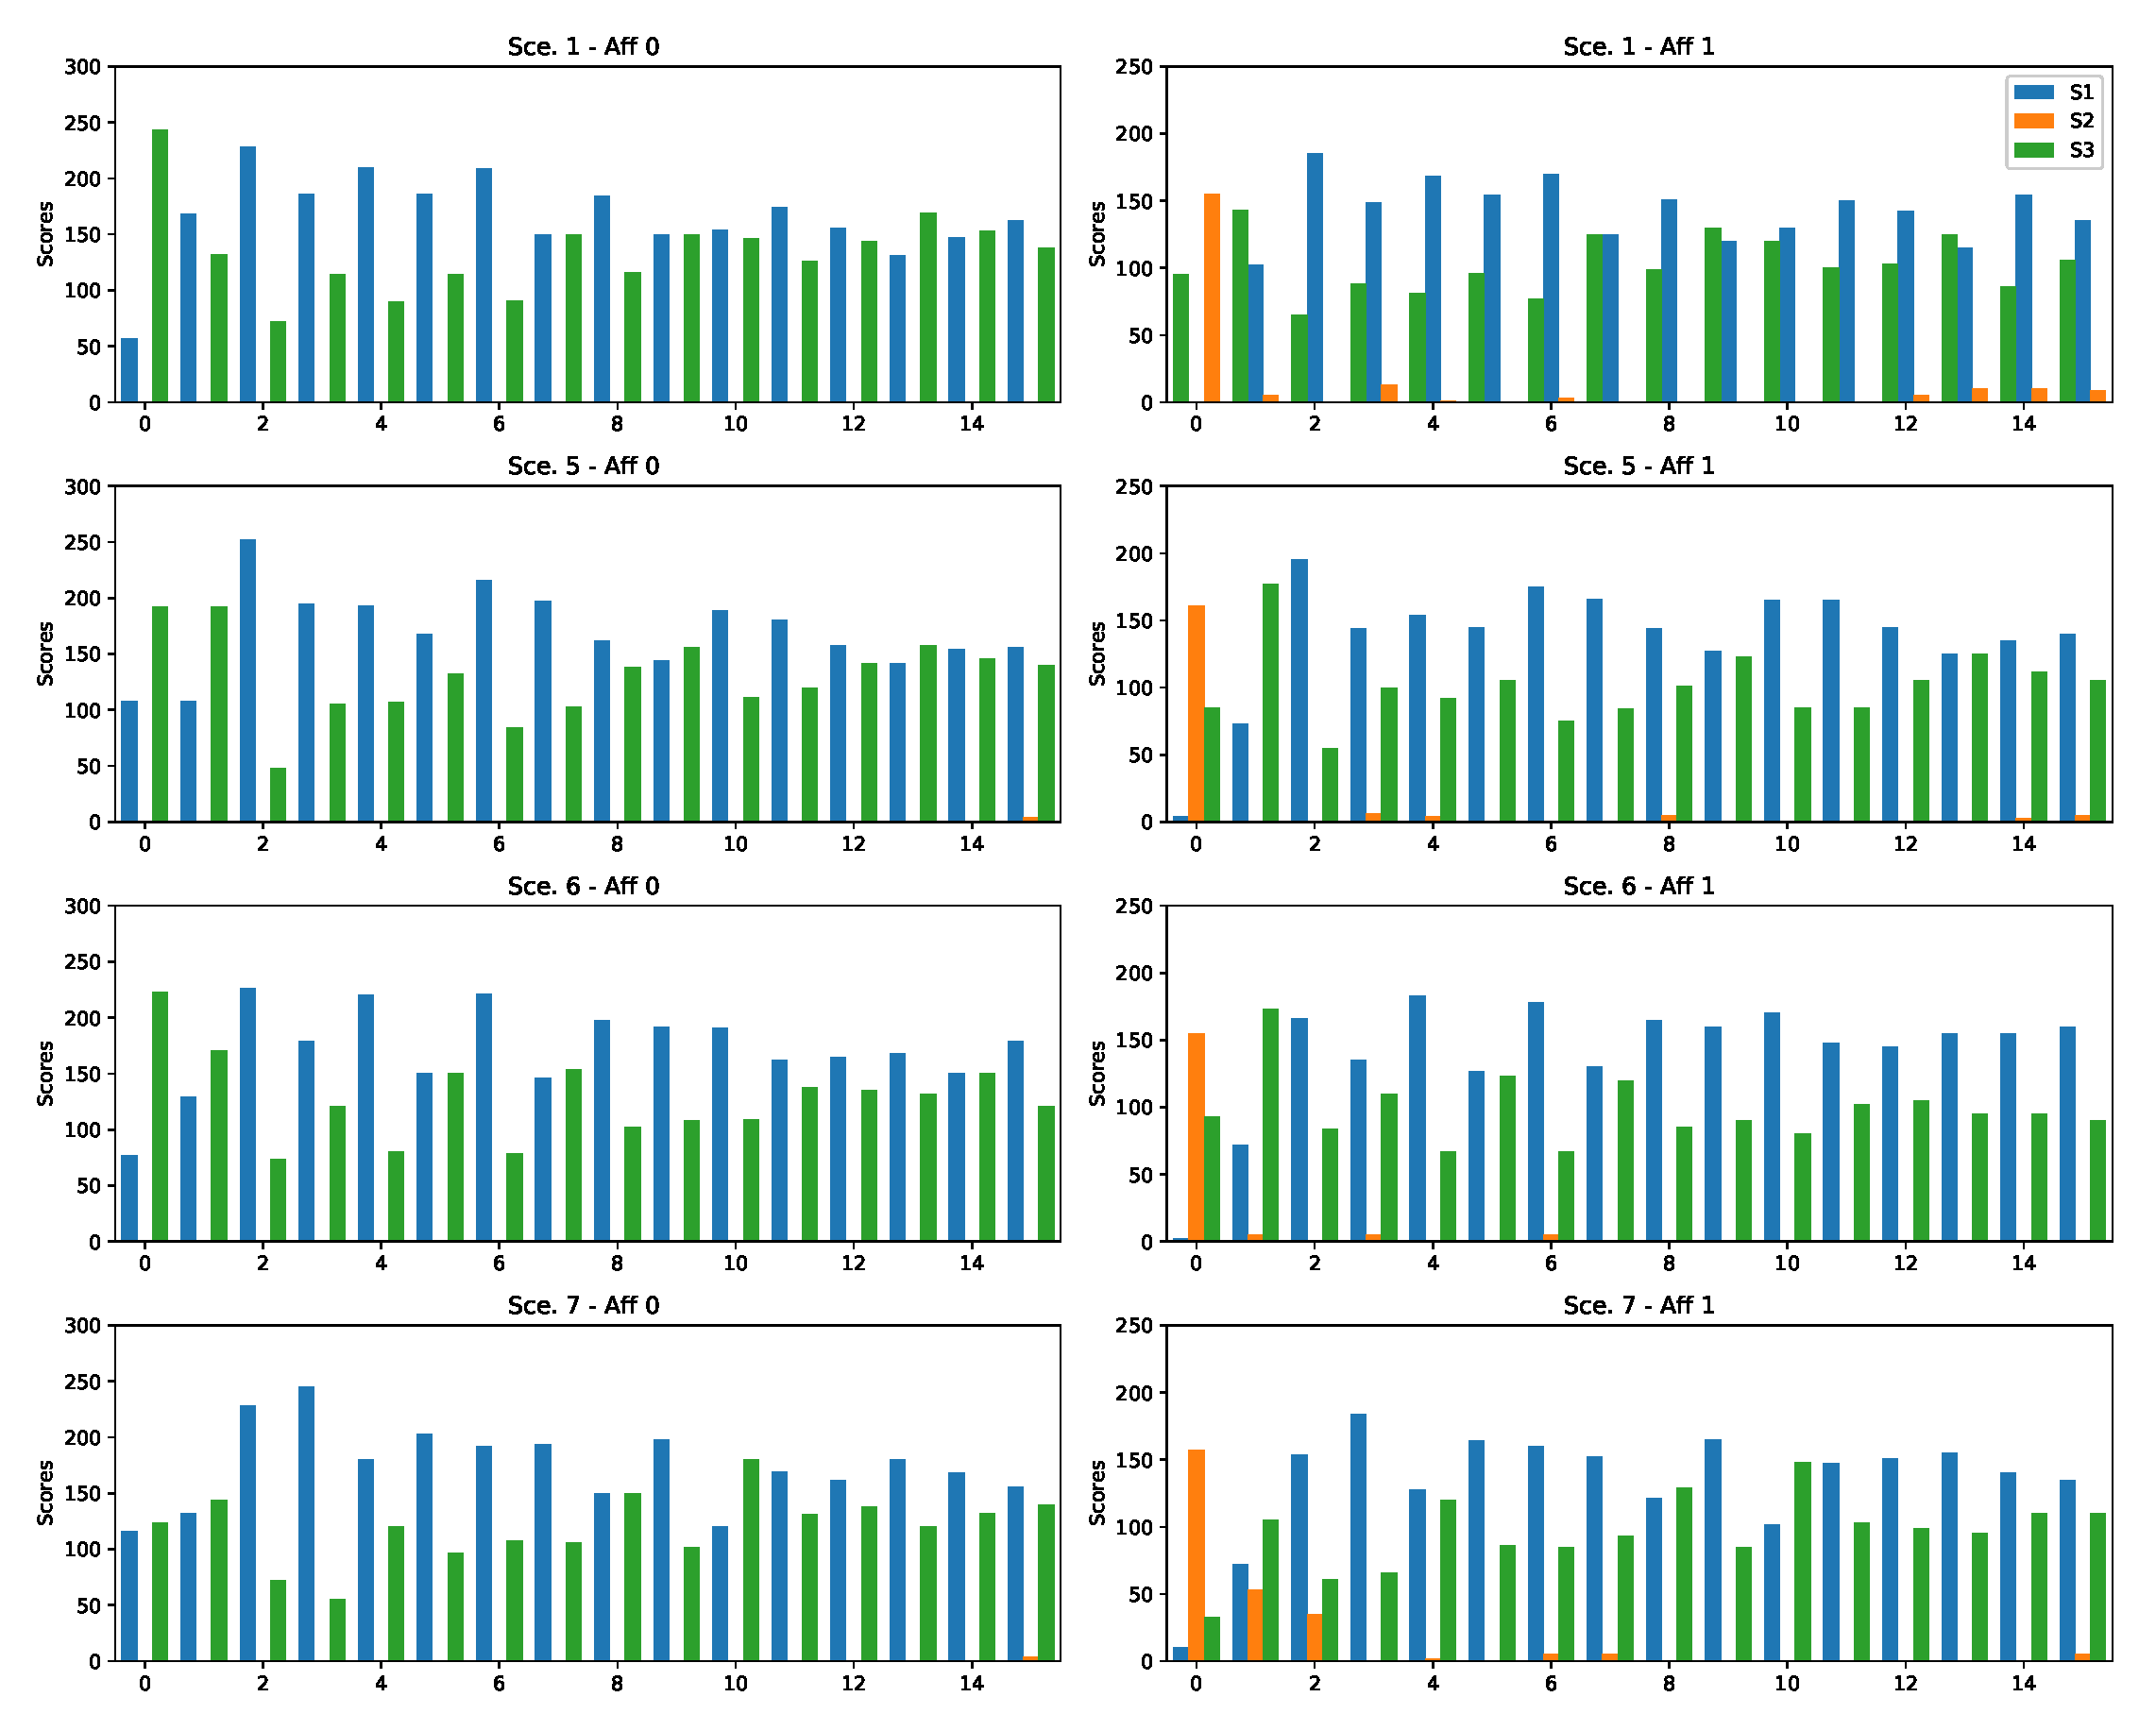
\includegraphics[width = 0.95\linewidth, angle = 0]{figures/PE_PL_SSelected_+Co}
\caption{Secondary issue selected.}
\label{fig:PE_PL_SSelected}
\end{figure}

\begin{figure}
\centering
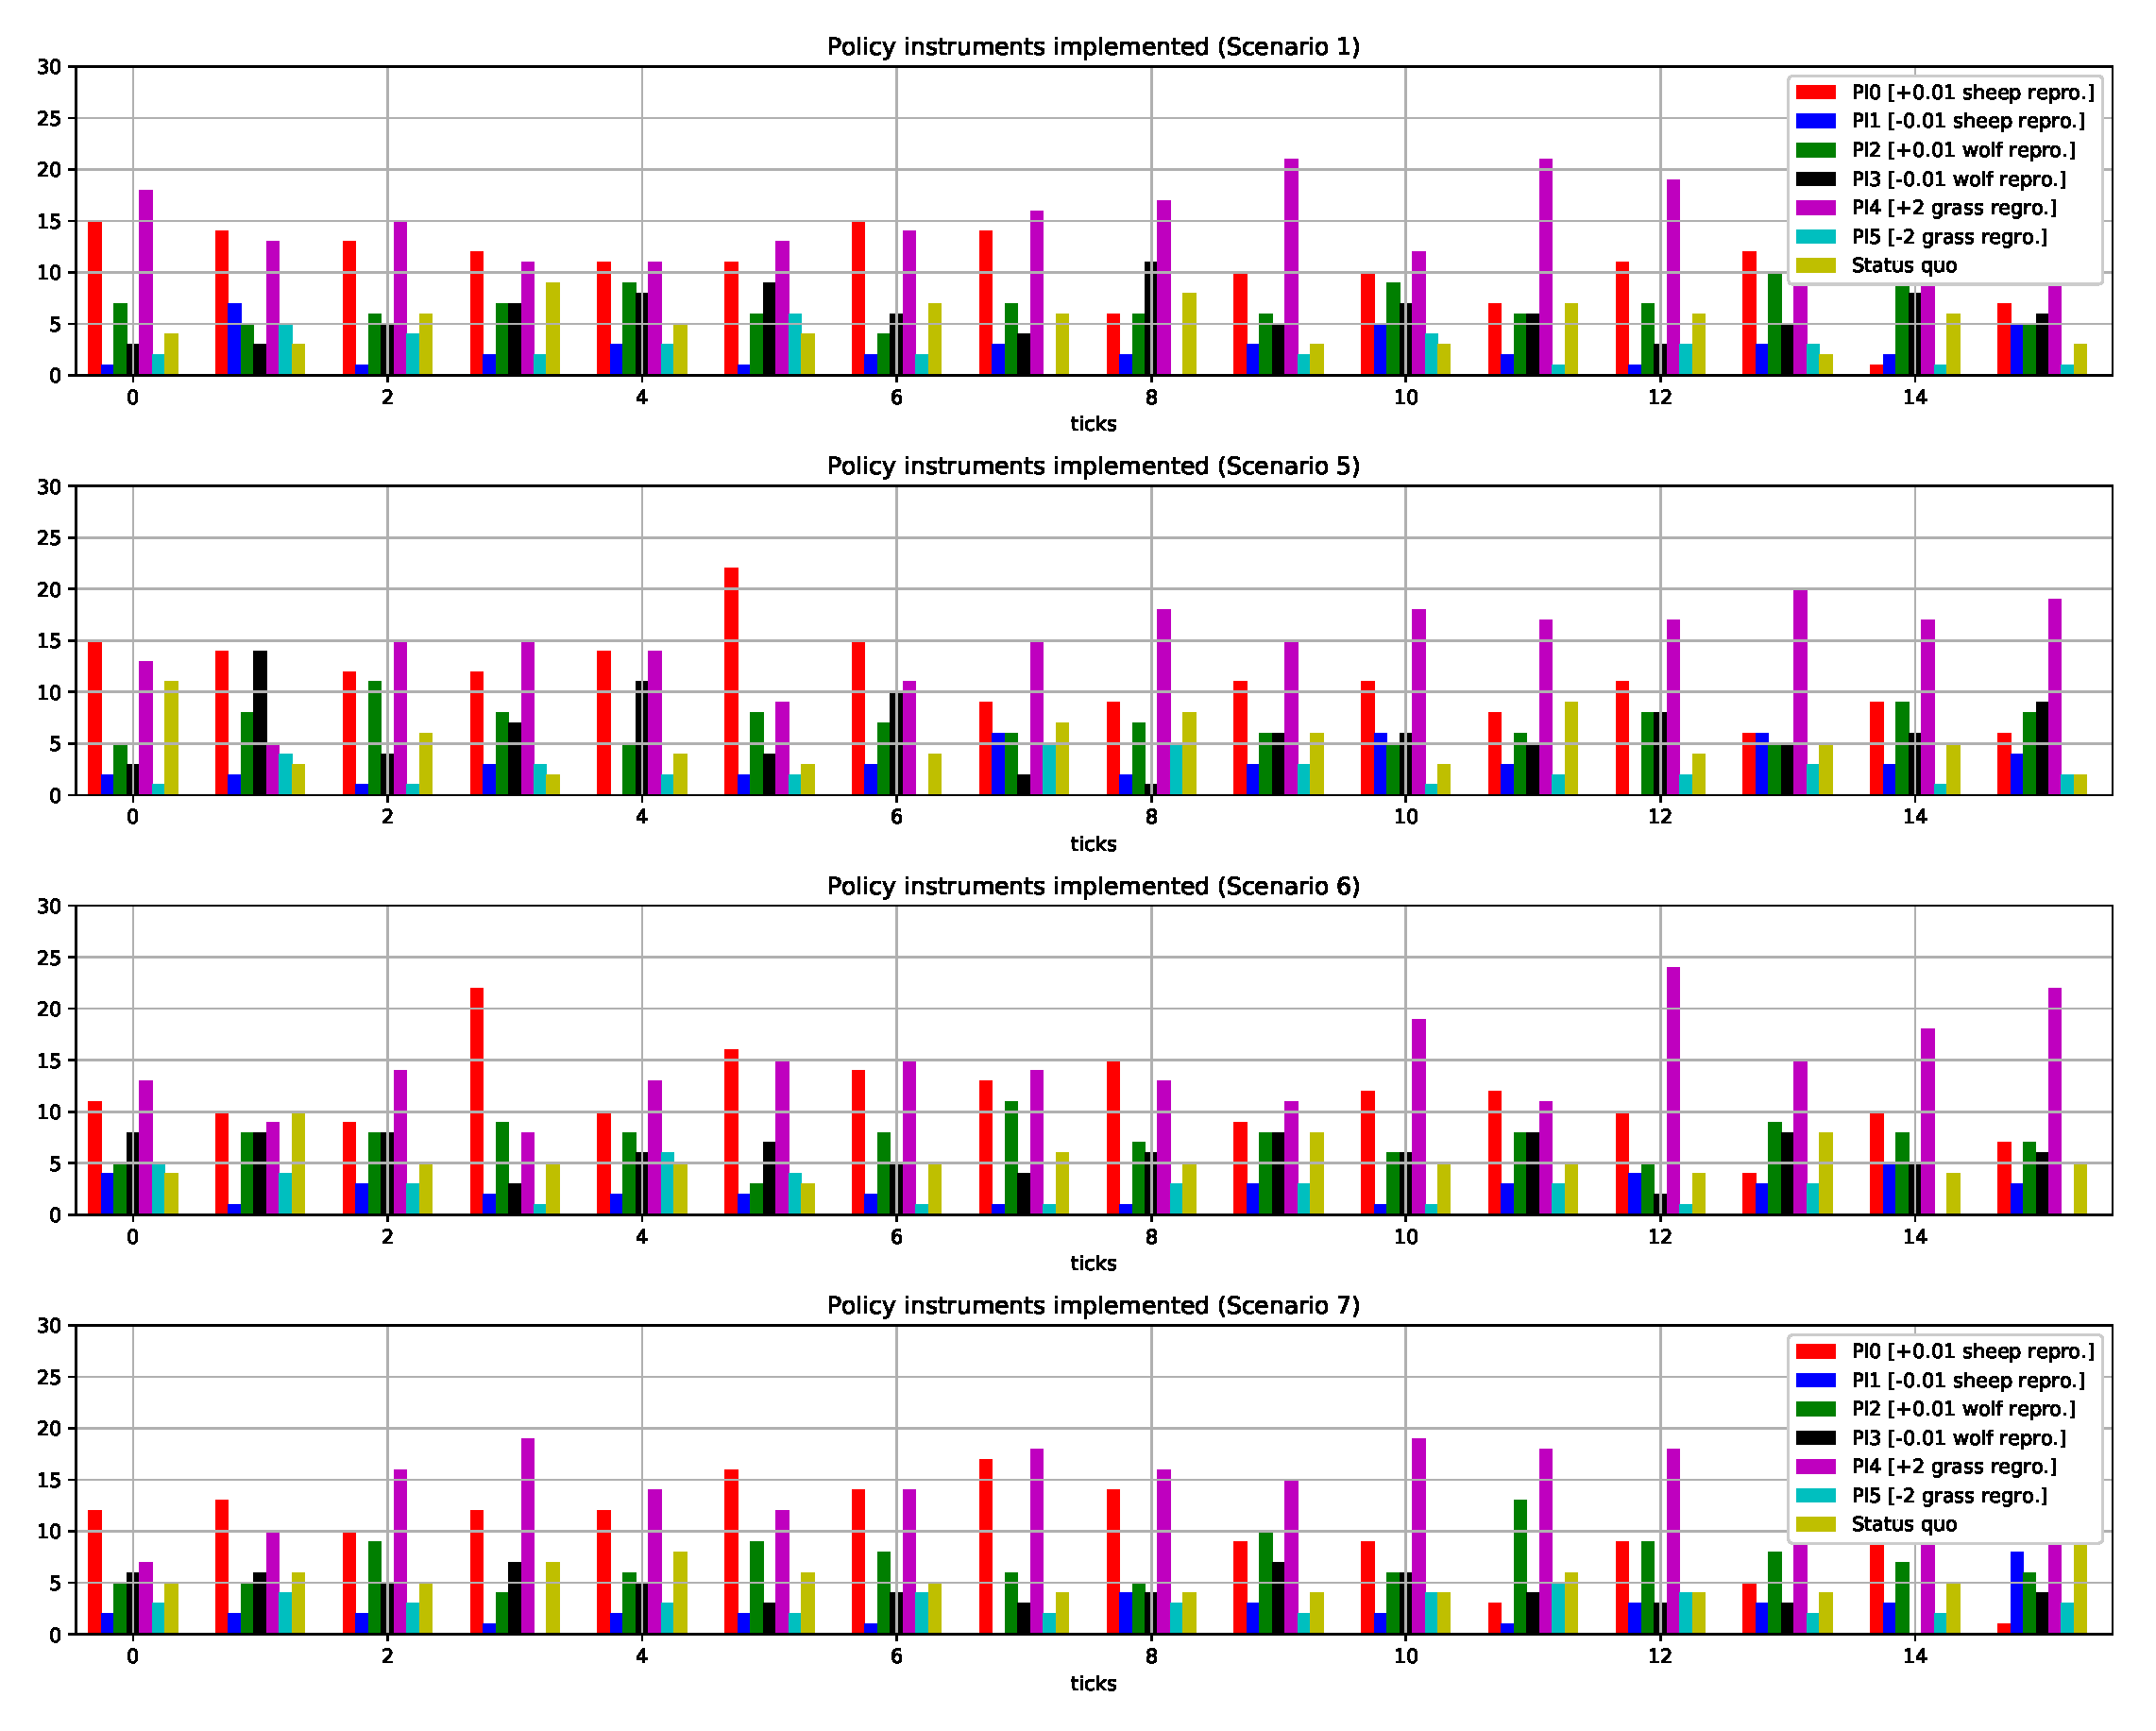
\includegraphics[width = 0.95\linewidth, angle = 0]{figures/PE_PI_selection_+Co}
\caption{Policy instruments selected.}
\label{fig:PE_PI_selection}
\end{figure}

\begin{figure}
\centering
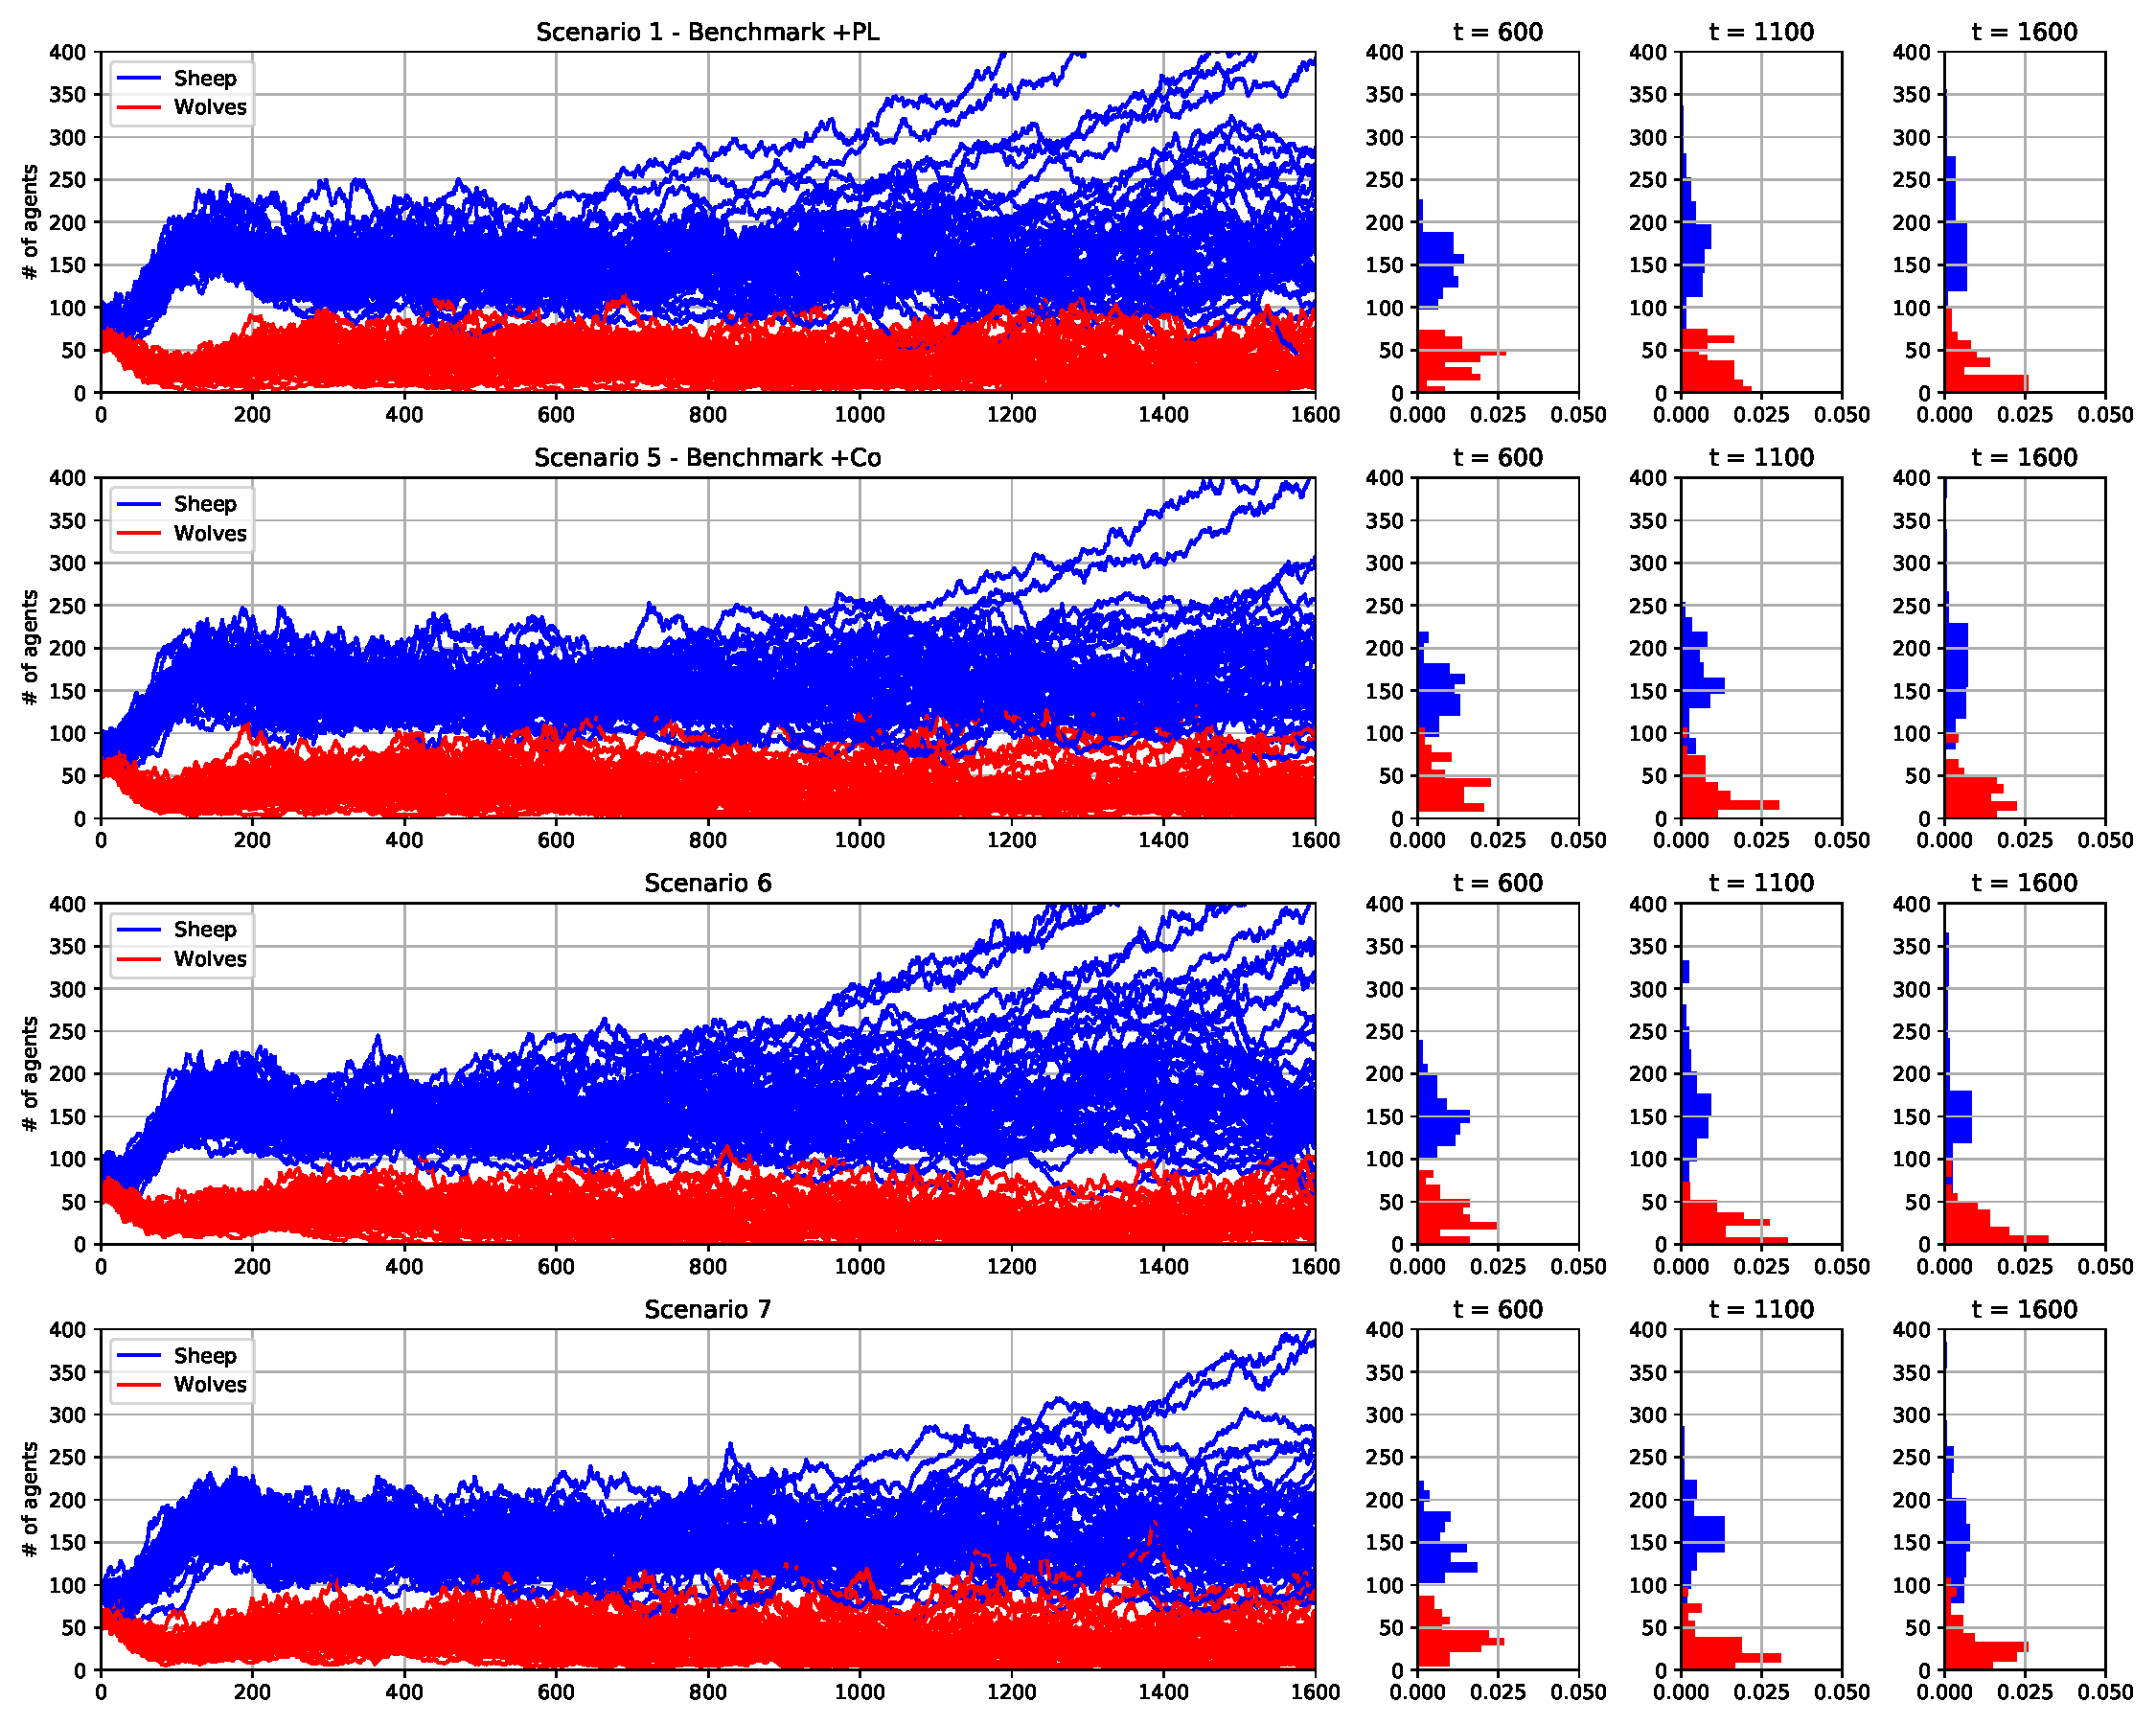
\includegraphics[width = 0.95\linewidth, angle = 0]{figures/Predation_Q1_popsWolfSheep_+Co}
\caption{Predation model results - wolf and sheep.}
\label{fig:Predation_Q1_popsWolfSheep}
\end{figure}

\begin{figure}
\centering
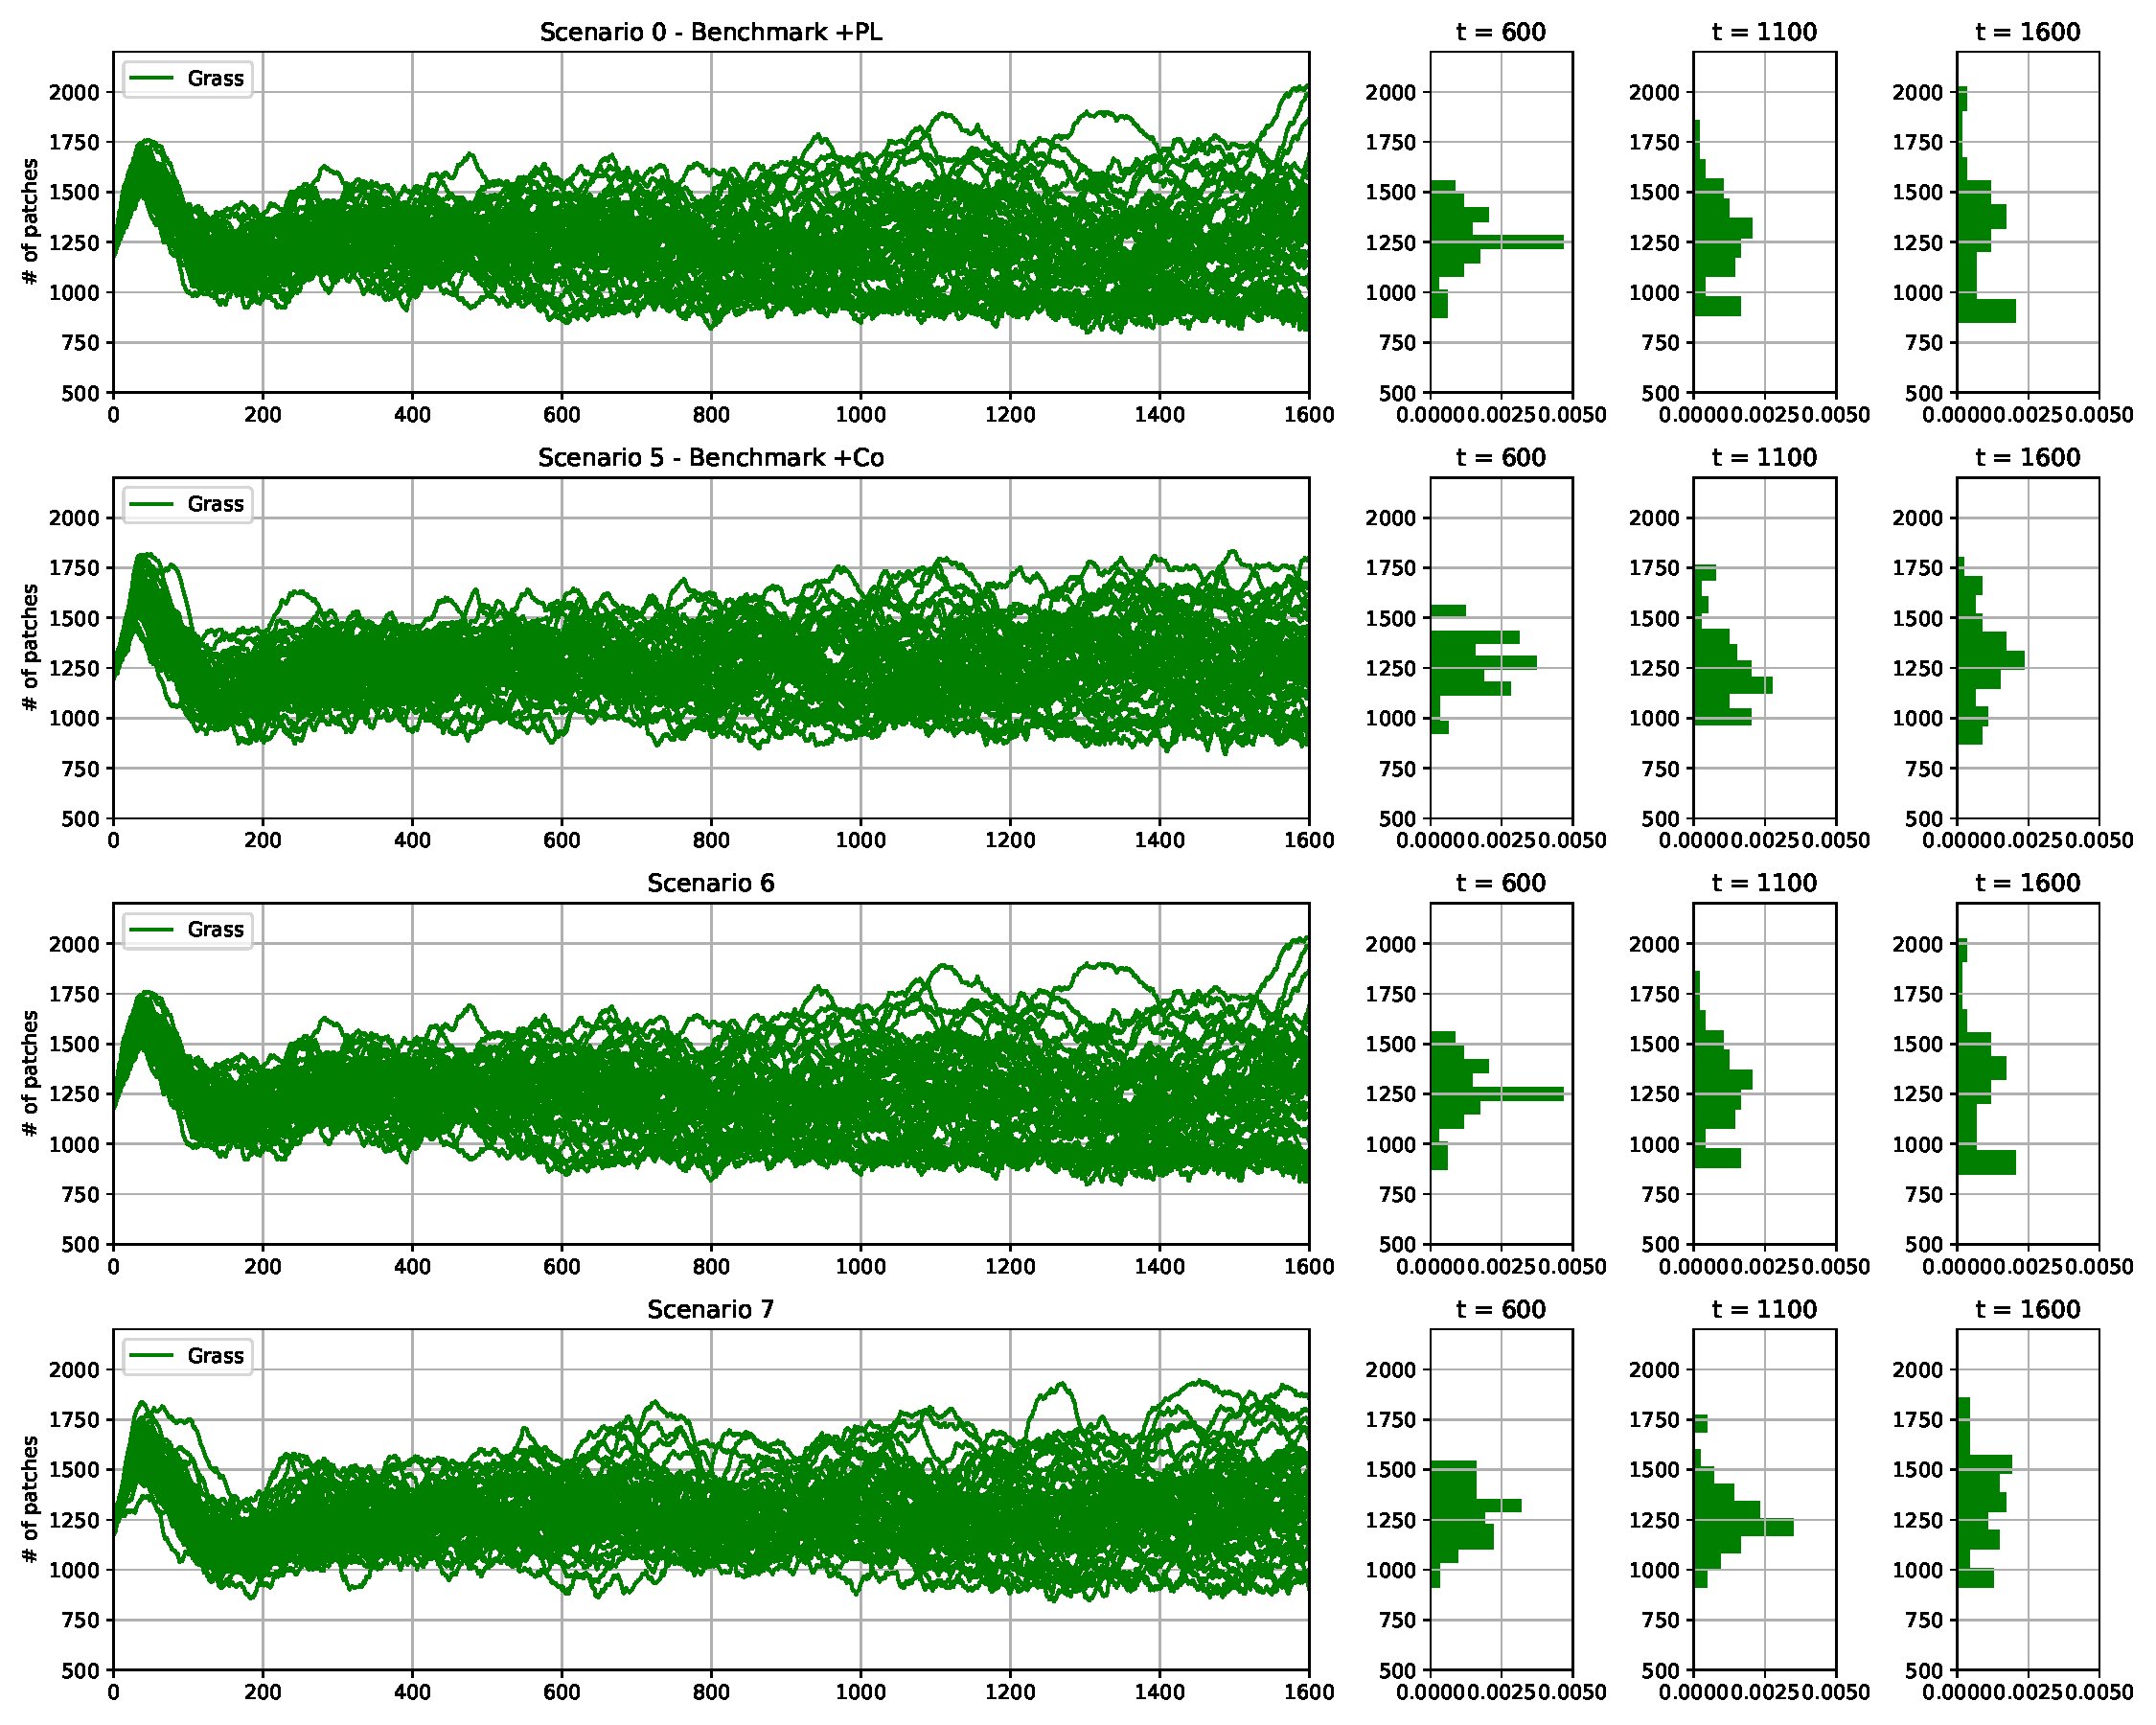
\includegraphics[width = 0.95\linewidth, angle = 0]{figures/Predation_Q1_popsGrass_+Co}
\caption{Predation model results - grass.}
\label{fig:Predation_Q1_popsGrass}
\end{figure}



%%%%%%%%%%%%%%%%%%%%%%%%%%%%%%%%%%%%%%%%%%%%%%%%%%%%%%%%%%%%%%%%%%
\bibliographystyle{apalike} 
\bibliography{references}
%%%%%%%%%%%%%%%%%%%%%%%%%%%%%%%%%%%%%%%%%%%%%


\end{document}
